\documentclass[../../main.tex]{subfiles}
\begin{document}
\chapter{Background Work}
\label{ch:background_work}

In this chapter, we delve into the foundational research areas central to this thesis. We begin by exploring how describing forms the basis for input into an animation system. Next, we discuss avatars as a key component of \gls{sl} synthesis. We then review the evolution of \gls{sl} descriptions, tracing their progression from linear \gls{glosses} to non-linear representations. Finally, we focus on the recent advancements in \gls{sl} synthesis, discussing various techniques and their implications for the field.

\section{Input: Sign Language Descriptions}
\label{ch:background_work:sign_language_descriptions}

A key challenge in \gls{sl} synthesis lies in the description of an \gls{sl} \gls{utterance} itself. The description of an \gls{utterance} answers essential questions such as:

\begin{itemize}
  \item \textbf{Body Motions}: What body motions create a meaningful \gls{sl} description?
  \item \textbf{Discourse Connection}: How do these motions connect to form a discourse?
  \item \textbf{Grammar and Syntax}: What are the grammatical and syntactical rules governing these signs?
  \item \textbf{Non-Manual Signals}: How can non-manual signals (such as facial expressions and body posture) be integrated with manual signs?
\end{itemize}

In this section, we first study the descriptive languages used to formalize \gls{sl} and how they describe body motions. These descriptions are crucial as they will be the input to the \gls{sl} synthesis system.

\subsection{Lexical Approaches to Creating a Discourse}
\label{ch:background_work:sign_language_descriptions:lexical_approaches}

Lexical approaches focus on individual signs and their components, such as handshapes, movements, and locations. These are essential for understanding the building blocks of \gls{sl} and how signs are produced. Some popular lexical descriptions include:

\subsubsection{Stokoe Notation}
\label{ch:background_work:sign_language_descriptions:lexical_approaches:stokoe_notation}

Stokoe Notation~\cite{stokoe1980sign} was developed to transcribe \gls{asl}. It breaks down signs into three main components: location, handshape, and movement (figure~\ref{fig:stokoe}). It is a simple and effective notation for basic transcription but focuses primarily on the manual components of signs.

\begin{figure}[h]
  \centering 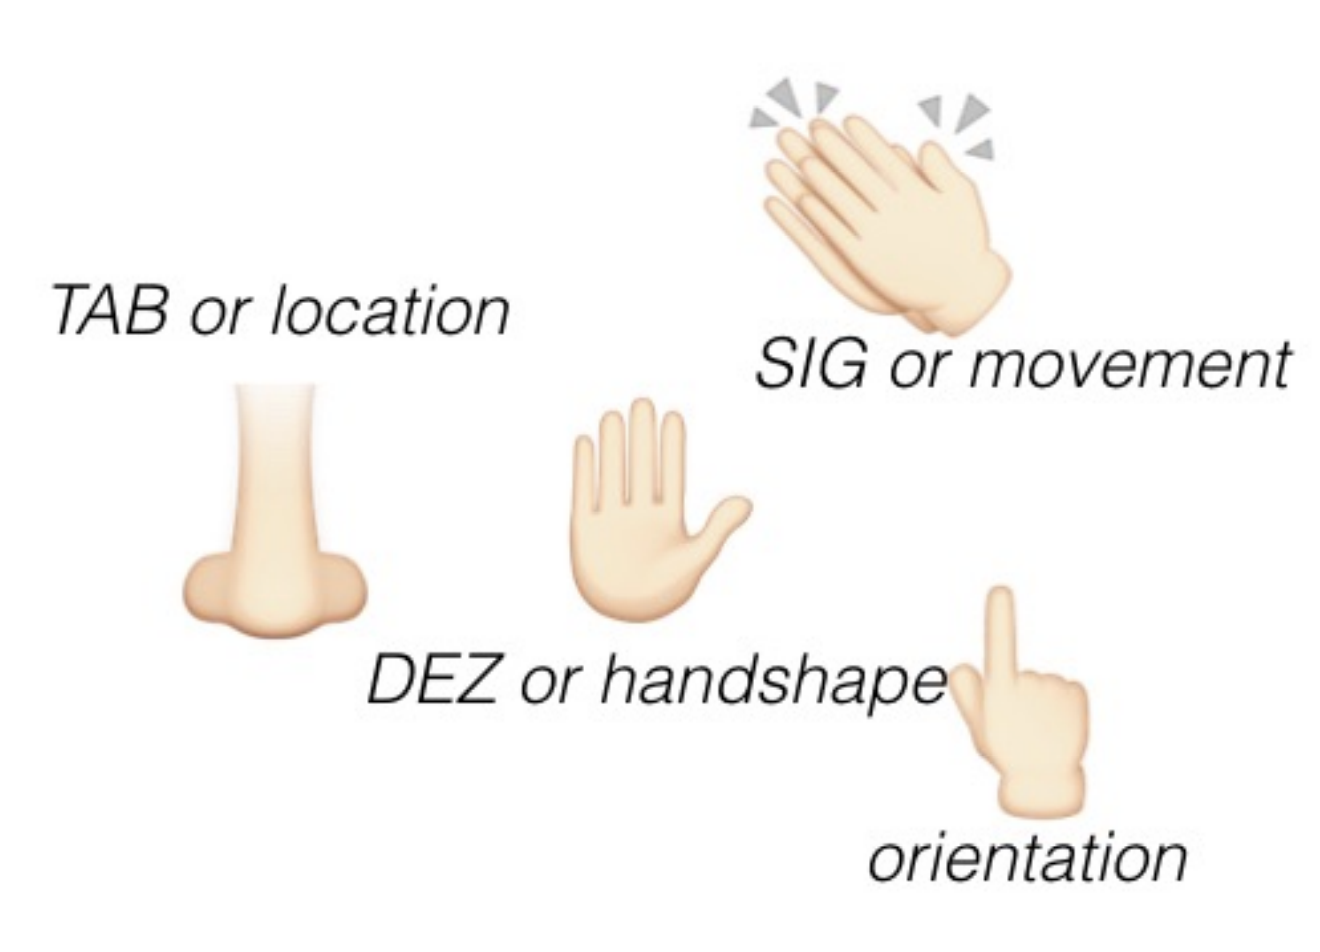
\includegraphics[width = 2.5in]{chapters/background_work/images/stokoe.png}
  \caption{Stokoe Notation}
  \label{fig:stokoe}
\end{figure}

\subsubsection{SignWriting}
\label{ch:background_work:sign_language_descriptions:lexical_approaches:signwriting}

SignWriting is a writing system developed by Valerie Sutton just after DanceWriting~\cite{sutton1973sutton} in the 1970s to represent \gls{sl} visually. It was later included as a part of the MovementWriting system. It is a featural script, representing the features of signs, such as handshapes, movements, and locations. SignWriting is designed to be easy to read and write, with symbols that resemble the gestures they represent. The script is written in two dimensions, with symbols arranged in a grid-like structure to capture various aspects of signs. Figure~\ref{fig:signwriting_coffee} shows an example of how the word "coffee" is represented in SignWriting. SignWriting has been used to transcribe over 40 \gls{sl}s worldwide and is recognized by the \gls{iswa} organization.

\begin{figure}[h]
  \centering 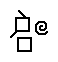
\includegraphics[width = 2.5in]{chapters/background_work/images/signwriting_coffee.png}
  \caption{Coffee in SignWriting}
  \label{fig:signwriting_coffee}
\end{figure}

\subsubsection{HamNoSys}
\label{ch:background_work:sign_language_descriptions:lexical_approaches:hamnosys}

The \gls{hamnosys} is a phonetic transcription system for documenting \gls{sl}s globally, developed in 1985 at the University of Hamburg. Unlike Stokoe's notation, which was specifically created for \gls{asl}, HamNoSys aims for broader application, transcending national \gls{hamnosys} boundaries. While Stokoe notation was later adapted to other \gls{sl}s, HamNoSys was designed from the outset to accommodate the diversity found in global \gls{sl}s.

The notation system employs nearly 200 symbols, organized into five primary categories, each capturing different aspects of a sign. These categories are Handshape, Hand Orientation, Hand Location, Movement, Symmetry Operator, and Non-Manual Markers. To describe a sign, a sequence of symbols is used, with each symbol corresponding to a specific feature. The symbols are arranged in a precise order: first, Handshape, followed by Hand Orientation, Hand Location, Movement, Symmetry Operator, and finally, Non-Manual Markers. This structured sequence allows for a clear and detailed representation of the sign. Figure~\ref{fig:hamnosys_coffee} shows how the word "coffee" is represented in HamNoSys.

HamNoSys offers a detailed representation of the nuanced components in an \gls{sl} \gls{utterance} rather than serving as a practical writing system. Its main purpose is linguistic, used primarily by linguists to analyze the specific features of individual signs. However, it has also found its applications in synthesis~\cite{elliott2010towards} as well as sign detection~\cite{mocialov2022unsupervised}.

\begin{figure}[h]
  \centering 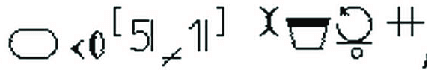
\includegraphics[width = 2.5in]{chapters/background_work/images/hamnosys_coffee.png}
  \caption{Coffee in HamNoSys}
  \label{fig:hamnosys_coffee}
\end{figure}

\subsection{AZee}
\label{ch:background_work:sign_language_descriptions:azee}

Even though these previously discussed lexical approaches are effective in capturing the individual components of signs, they are limited in their ability to represent the dynamic and context-sensitive nature of \gls{sl} discourse. This is because they simplify signs as \gls{glosses}. As a reason, their applications in \gls{sl} synthesis are limited. The AZee model, however, is grounded in the concept of production rules, which link specific meanings to observable forms. This model operates on the principle that the meaning of a sign can be broken down into a set of features, which are then represented through production rules. These rules guide the generation of the sign's form, encompassing aspects like handshape, movement, and location. Designed to be both flexible and extensible, the AZee model is capable of representing a broad spectrum of signs and \gls{sl}s. It is particularly advantageous for \gls{sl} synthesis, offering a systematic and structured method for describing signs and their components.

\subsubsection{Representation of an \gls{utterance} in AZee}
\label{ch:background_work:sign_language_descriptions:azee:representation}

The AZee model uses a hierarchical structure to represent signs, with each level capturing different aspects of the sign. At the lowest level, the model describes the physical form of the sign, such as handshapes, movements, and locations. These physical forms are then combined to create more complex signs, forming a hierarchical structure that mirrors the linguistic structure of the sign. To understand this better, consider the example of the \gls{utterance} "a person aged 52" in \gls{lsf} from the \emph{1R-JP} discourse from the 40 brèves corpus~\cite{challant2022first}. The AZee code for this \gls{utterance} would be:

\begin{verbatim}
  :info-about
    'topic
    :personne
    'info
    :info-about
      'topic
      :âge
      'info
      :tens-units
        'tens
        .nb-5
        'units
        .nb-2
\end{verbatim}

The \gls{azee_interpreter} parses this description recursively, generating an \gls{azee_score}. An \gls{azee_score} being recursive in nature can contain other \gls{azee_score}s. The figure~\ref{fig:azee_score_example} shows the recursive structure for the \gls{utterance} "a person aged 52" using the AZee model. Each of the blocks in the figure represents an \gls{azee_score} .

\begin{figure}[h]
  \centering 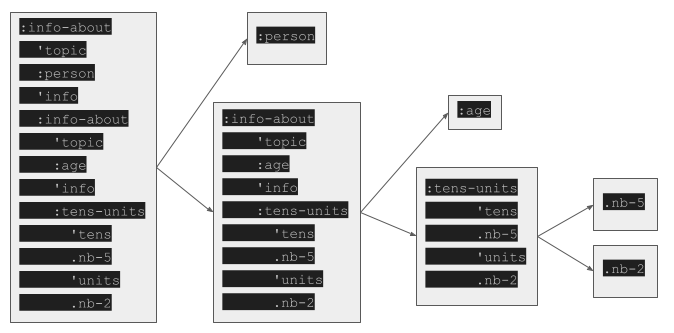
\includegraphics[width = 5in]{chapters/background_work/images/azee_score_example.png}
  \caption{AZee's recursive score representation for the utterance "a person aged 52"}
  \label{fig:azee_score_example}
\end{figure}

Note that the \gls{azee_score} representation also gives us temporal information about the \gls{utterance}. Such a detailed representation is important to us as it can help in creation of a timeline and will also be the input for our \gls{sl} synthesis system. 

\subsubsection{Low-Level Descriptions in AZee}
\label{ch:background_work:sign_language_descriptions:azee:low_level}

Apart from the high-level representation of an \gls{utterance} as shown in figure ~\ref{fig:azee_score_example}, the AZee model also supports low-level descriptions that directly correlate with the postures of an abstract avatar. This low-level description is also a recursive \gls{azee_score} and contains a set of \gls{cstr_score}s. A \gls{cstr_score} is a score which contains a set of \gls{posture_constraint}s on the posture that capture various components of the utterance, such as handshapes, movements, and locations. For example, let's consider the \gls{azee_score} for \emph{:personne} (person in \gls{lsf}, figure~\ref{fig:person_lsf}) in the above utterance. Figure ~\ref{fig:azee_score_person} shows the low-level description for this \gls{azee_score}. It contains 4 \gls{cstr_score}s, \emph{HAND\_START}, \emph{HAND\_END}, \emph{HAND\_PATH}, and \emph{PERM}, each containing \gls{posture_constraint}s on the posture of the avatar.

\begin{figure}
  \centering 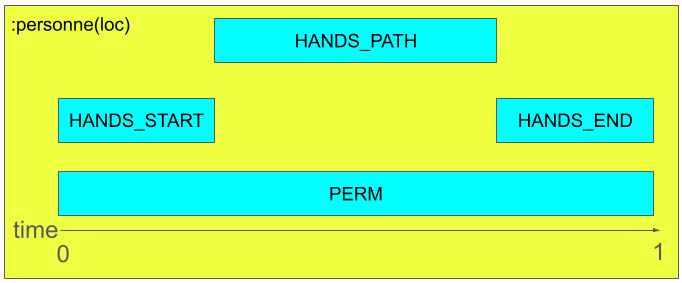
\includegraphics[width = 4in]{chapters/background_work/images/azee_score_person.png}
  \caption{Low-level description for \emph{:personne}}
  \label{fig:azee_score_person}
\end{figure}

\begin{figure}
  \centering 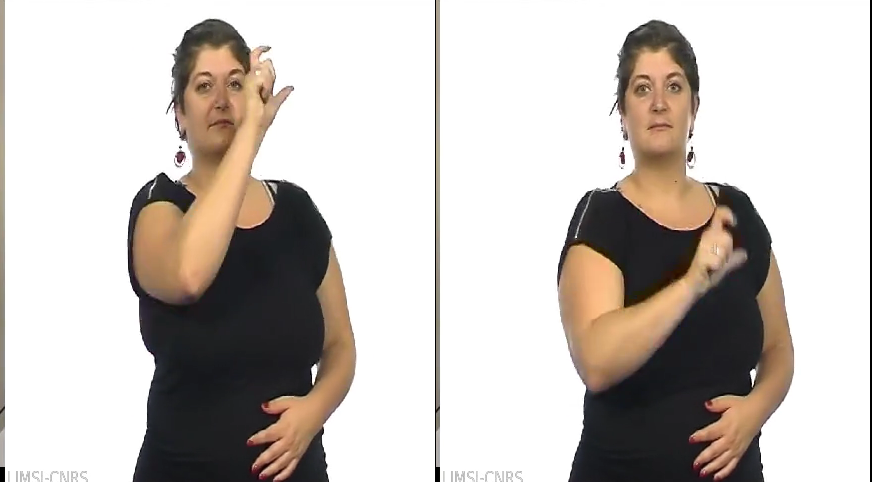
\includegraphics[width = 3.5in]{chapters/background_work/images/person_lsf.png}
  \caption{Person in French Sign Language}
  \label{fig:person_lsf}
\end{figure}

\emph{HAND\_START} and \emph{HAND\_END} represent the hands placements and orientations at the start and end of the sign, respectively. \emph{HAND\_PATH} captures the trajectory of the head during the sign, while \emph{PERM} contains the permanent features which are active throughout the duration (in this case, closed middle, ring and pinky fingers while the thumb and index are partially open).

An \gls{azee_score} can be of various types. These include:

\begin{itemize}
  \item \textbf{Synced Score}: A recrusive structure containing other scores with some relative timing information (figure~\ref{fig:azee_score_example}).
  \item \textbf{\gls{cstr_score}}: A score specifying \gls{posture_constraint}s on the body parts (figure~\ref{fig:azee_score_person}).
  \item \textbf{Hold Score}: A score holding another score for some amount of time.
  \item \textbf{KeyFrame Score}: An abstract \emph{flattened} representation of a \gls{cstr_score}.
  \item \textbf{Non-Animated KeyFrame Score}: A \emph{flattened} representation of \gls{posture_constraint}s on body parts per frame.
  \item \textbf{Animated KeyFrame Score}: A \emph{flattened} representation of pose changes per frame.
\end{itemize}

Similarly, \gls{posture_constraint}s in a \gls{cstr_score} can be of various types. These include:

\begin{itemize}
  \item \textbf{Place}: Constrains a body \gls{site} to be placed at a specific location in 3D space.
  \item \textbf{Orient}: Constraints the orientation of a bone.
  \item \textbf{Morph}: Constrains a morphological change of a body part(s).
  \item \textbf{Transpath}: Constrains a body \gls{site} along a path.
  \item \textbf{Look-At}: Constrains the body to look at a specific point.
  \item \textbf{Trill}: Shaking of a body part along an axis.
\end{itemize}

In addition to these, the AZee model includes several other important operators and concepts that allows to represent \gls{sl}. Some of these include,

\begin{itemize}
  \item \textbf{Dynamic Points and Paths}: to define moving targets or locations that body parts should follow.
  \item \textbf{3D math operations}: Various math operations such as vectors, mathematical curves, and transformations are supported in AZee.
  \item \textbf{Partial Application of Operators}: allows for the partial application of an operator to a set of arguments, effectively creating a new operator.
\end{itemize}

\subsubsection{AZee Templates}
\label{ch:background_work:sign_language_descriptions:azee:templates}

AZee also allows for use of templates which are abstract representations of a \gls{sl} utterance, linking linguistic descriptions with animated motions. For example, an AZee template like \emph{:info-about(:âge,?info)} could match an AZee expression such as \emph{:info-about(:âge,:tens-units(:five,:two))}, where the variable \emph{info} would be assigned the function \emph{:tens-units(:five,:two)}. This template can be used to procedurally create animations, where the person's age (52, in this case) is dynamically inserted based on the template match.

Lastly, an AZee description can also be drawn in the form of \gls{svg} images using AZVD~\cite{filhol2024software}. Figure~\ref{fig:azvd} shows the visual description for the \gls{utterance} "a person aged 52".

\begin{figure}
  \centering 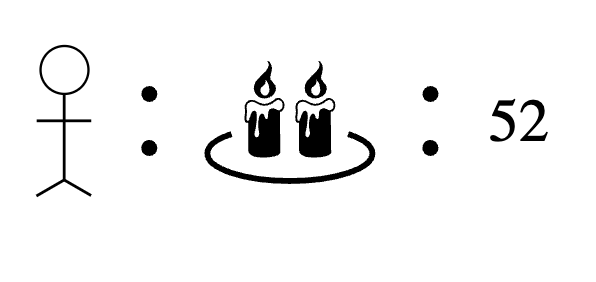
\includegraphics[width = 2.5in]{chapters/background_work/images/azvd.png}
  \caption{AZee visual description for a person aged 52}
  \label{fig:azvd}
\end{figure}

All of these features make the AZee model a powerful tool and a suitable input for our \gls{sl} synthesis system.

\section{Sign Language Synthesis}
\label{ch:background_work:sign_language_synthesis}

\gls{sl} synthesis is the process of generating \gls{sl} discourses from linguistic input. This process involves resolving a linguistic description on a digital human. This can be in the form of handshapes, movements, facial expressions, etc. \gls{sl} synthesis is a complex and interdisciplinary field that draws on linguistics, computer science, animation, and human-computer interaction. Several approaches have been developed to synthesize \gls{sl} animations, each with its unique strengths and challenges.

\subsection{2D Techniques}
\label{ch:background_work:sign_language_synthesis:2d_techniques}

Various 2D synthesis~\cite{jiang2024signclipconnectingtextsign, moryossef2024signmtrealtimemultilingualsign} already exist which generate signs directly from \gls{glosses}. One of the newer techniques~\cite{walsh2024sign} addresses the common issue of regression to the mean in previous models, which often resulted in unnatural and under-articulated signing. The authors propose a method called "sign stitching," which involves normalizing signs into a canonical pose, cropping, stitching them together, and applying frequency domain filtering and resampling to produce cohesive, expressive \gls{sl} sequences. They also introduce a \gls{nsvq} transformer to integrate facial expressions, enhancing the naturalness of the signs. The approach is evaluated using a SignGAN model~\cite{saunders2020everybodysignnowtranslating} to generate photo-realistic signers, achieving state-of-the-art performance across multiple datasets and receiving positive feedback in user evaluations for its realism and expressiveness.

Figures~\ref{fig:synthesis_mediaipe_2d} and~\ref{fig:synthesis_gan_2d} illustrate how the output of such methods usually look like, showing the initial mediapipe-based synthesis and the subsequent fitting of a GAN on the Mediapipe skeleton to enhance the realism of the generated signs.

\begin{figure}
  \centering 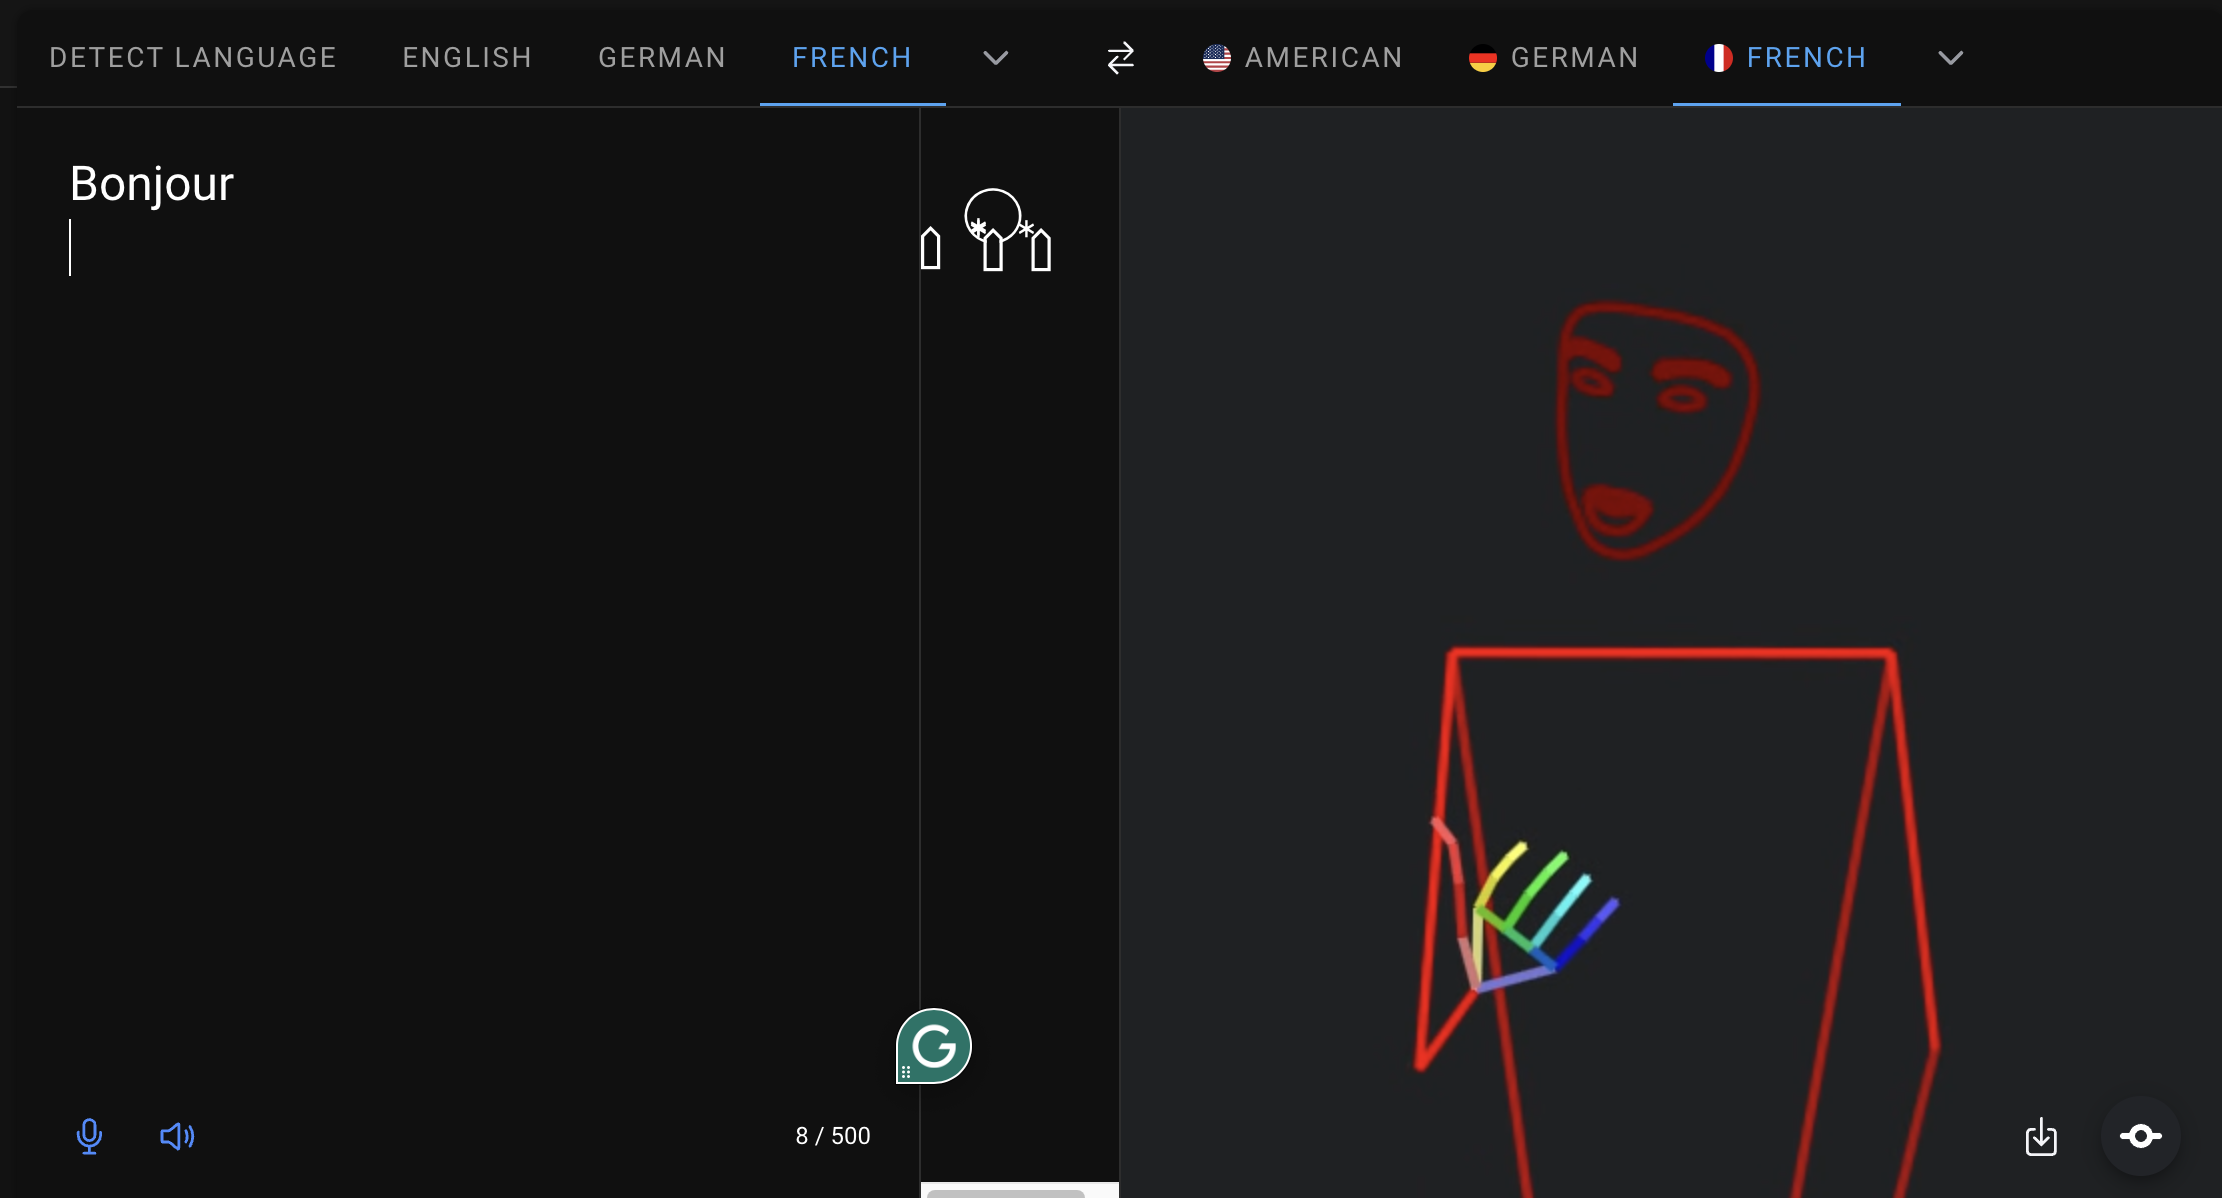
\includegraphics[width = 2.5in]{chapters/background_work/images/sign_writing_synthesis.png} 
  \caption{Synthesis using Sign-Stitching} 
  \label{fig:synthesis_mediaipe_2d} 
\end{figure}

\begin{figure} 
  \centering 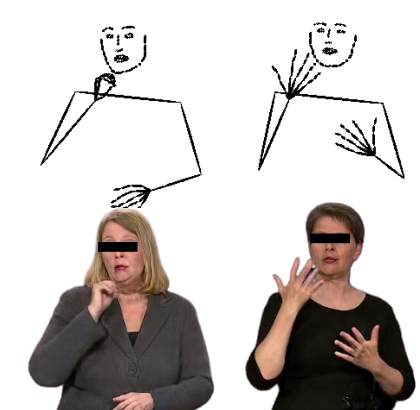
\includegraphics[width = 2.5in]{chapters/background_work/images/gan_synthesis.png} 
  \caption{SignGAN~\cite{saunders2020everybodysignnowtranslating}} 
  \label{fig:synthesis_gan_2d} 
\end{figure}

While such techniques are computationally less demanding during inference. Require a large amount of data to train the model. They also lack the depth and realism of 3D animations and struggle with capturing complex spatial relationships in \gls{sl}.

\subsection{3D Techniques}
\label{ch:background_work:sign_language_synthesis:3d_techniques}

3D techniques generate \gls{sl} animations using avatars that operate in a three-dimensional space. These methods provide a more immersive and realistic representation of \gls{sl}. 3D synthesis can leverage advanced avatars, such as those created by MetaHuman or SMPL-X, to achieve high levels of detail and expressiveness. Avatars are digital representations of characters or individuals, and are quite poular in in \gls{sl} synthesis to animate the described signs. This subsection explores the components of avatar creation and animation, followed by their use in \gls{sl} synthesis.

\subsubsection{Skeleton}
\label{ch:background_work:sign_language_synthesis:3d_techniques:skeleton}

The skeleton of a digital avatar is a crucial component for enabling realistic movement and animation. It consists of a hierarchical structure of bones, joints that mimic the human skeletal system. This section explores several popular skeleton systems used in avatar creation and animation.

\paragraph{Mixamo}
\label{ch:background_work:sign_language_synthesis:3d_techniques:skeleton:mixamo}

Mixamo is a widely used online platform that provides a vast library of pre-rigged 3D characters and animations. Developed by Adobe, Mixamo offers an easy-to-use interface where users can upload their 3D models and automatically rig(add skeleton and other controllable features) them using Mixamo's auto-rigging tool. This tool identifies keypoints on the model and generates a skeleton with appropriate bone placements. Additionally, Mixamo offers a range of pre-made animations that can be applied to the rigged models, facilitating quick and efficient animation workflows. The platform supports various file formats and is compatible with many 3D software tools. A standard Mixamo skeleton consists of 65 bones, covering major body parts, including the spine, arms, legs, hands, and head. Figure~\ref{fig:mixamo_autorigging} shows the process of auto-rigging a 3D model using Mixamo, while Figure~\ref{fig:mixamo_skeleton} illustrates the standard Mixamo skeleton structure.

\begin{figure} 
  \centering 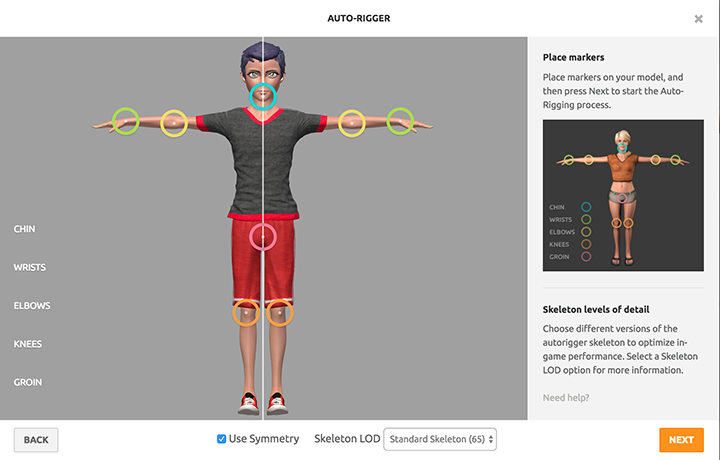
\includegraphics[width = 2.5in]{chapters/background_work/images/mixamo_autorigging.png} 
  \caption{Autorigging using Mixamo} 
  \label{fig:mixamo_autorigging} 
\end{figure}

\begin{figure} 
  \centering 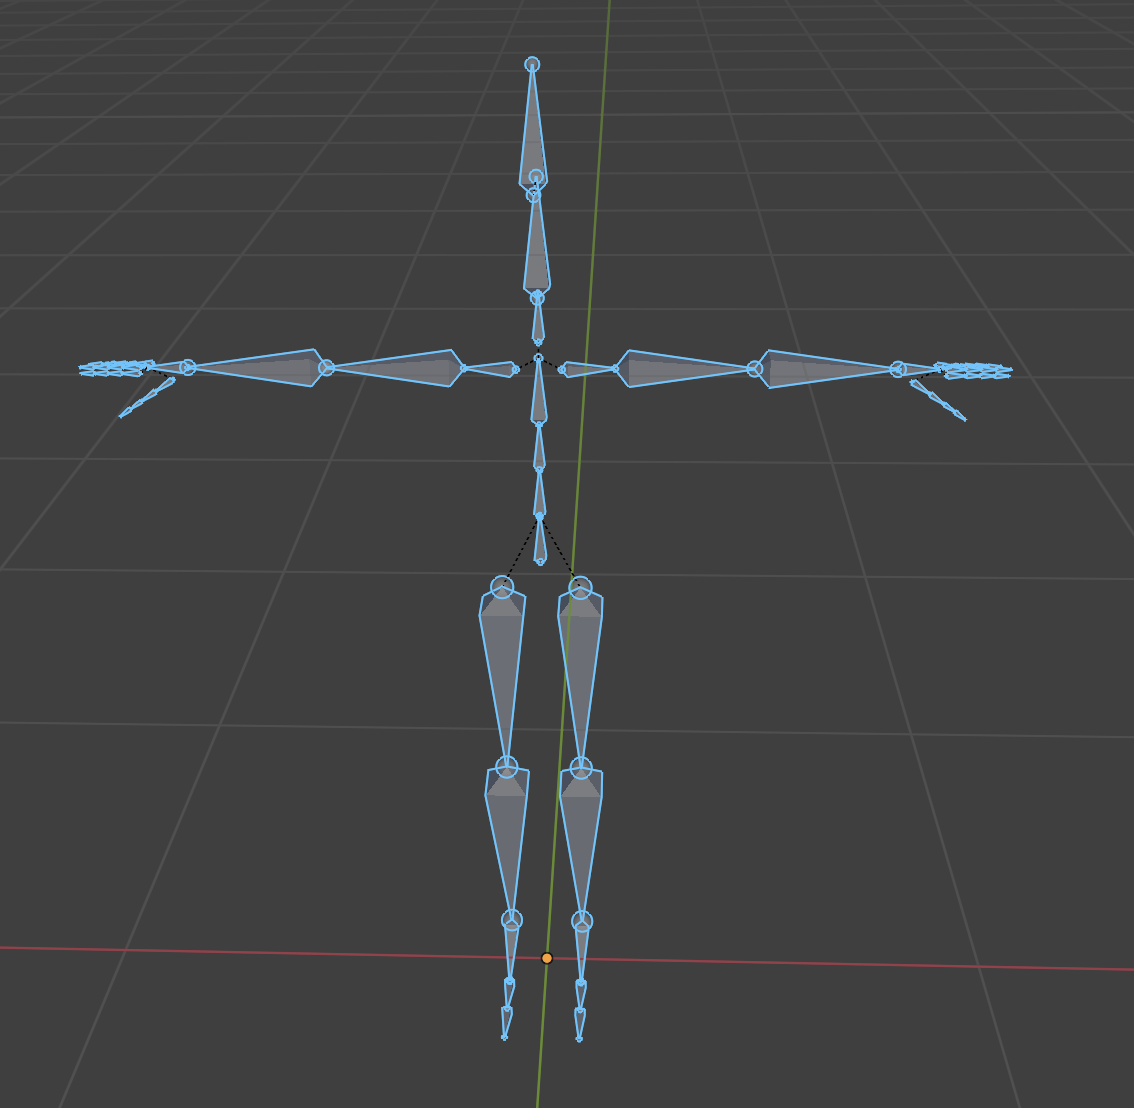
\includegraphics[width = 2.5in]{chapters/background_work/images/mixamo_skeleton.png} 
  \caption{Standard Mixamo skeleton structure} 
  \label{fig:mixamo_skeleton} 
\end{figure}

\paragraph{SMPL-X}
\label{ch:background_work:sign_language_synthesis:3d_techniques:skeleton:smpl_x}

\gls{smplx} is a state-of-the-art parametric model for generating highly detailed and anatomically accurate 3D human avatars. SMPL-X encodes the shape and pose of a character using a low-dimensional space, allowing for efficient representation and manipulation. Thus, a configuration of about 100 numbers can represent the pose as well as the shape of the avatar. The hierarchy of a SMPL-X skeleton is shown in figure~\ref{fig:smpl_x_skeleton}, and the corresponding \gls{latent_space} representation in figure~\ref{fig:latent_space_smplx}.

\begin{figure} 
  \centering 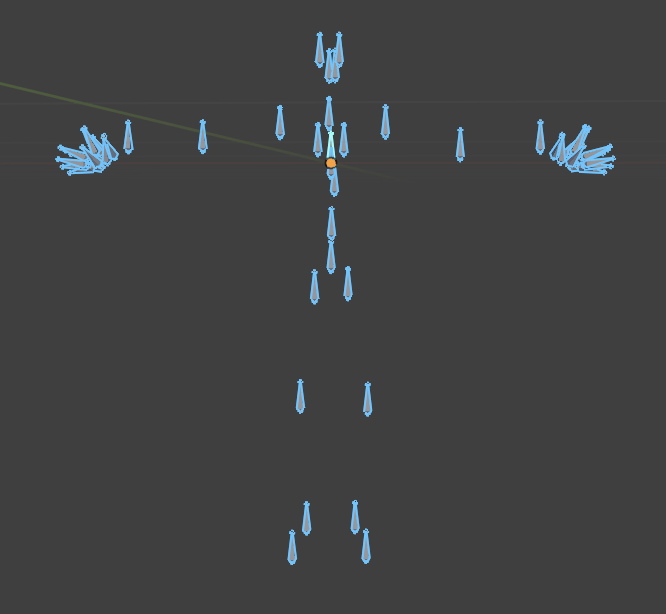
\includegraphics[width = 2.5in]{chapters/background_work/images/smpl_x_skeleton.png} 
  \caption{SMPL-X skeleton} 
  \label{fig:smpl_x_skeleton} 
\end{figure}

\begin{figure} 
  \centering 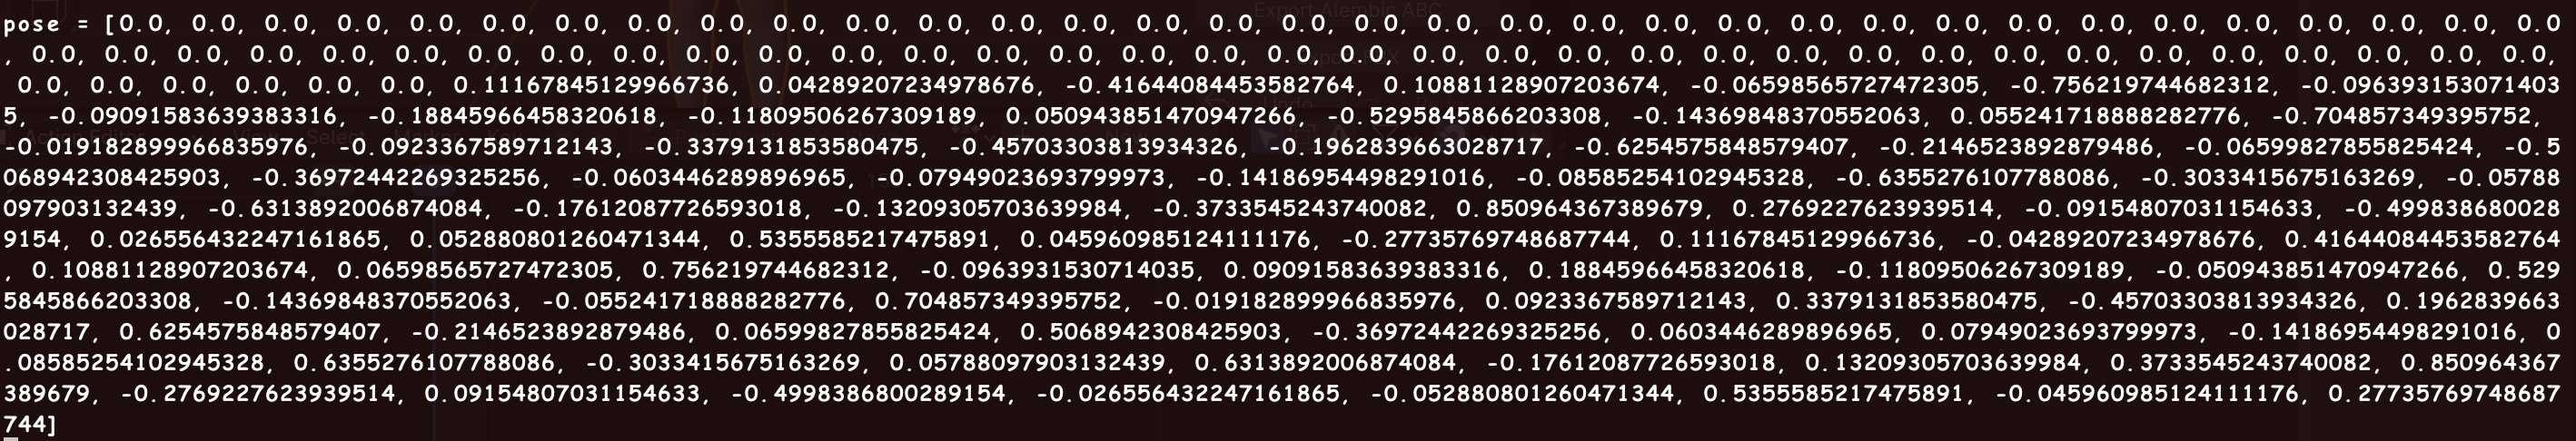
\includegraphics[width = 2.5in]{chapters/background_work/images/latent_space_smplx.png} 
  \caption{SMPL-X latent space} 
  \label{fig:latent_space_smplx} 
\end{figure}

\subsubsection{Mesh and Texture}
\label{ch:background_work:sign_language_synthesis:3d_techniques:mesh_and_texture}

The mesh of a digital avatar is the 3D model that forms the surface representation of the character. It consists of vertices, edges, and faces that define the shape and structure of the avatar. Creating and manipulating meshes is a fundamental aspect of 3D modeling and animation, allowing for detailed and realistic character designs.

Textures are 2D images applied to the surface of a 3D model to enhance its appearance and realism. Textures can represent various surface properties such as color, roughness, reflectivity, and transparency. Common types of textures include diffuse maps (color), specular maps (reflectivity), normal maps (surface detail), and roughness maps (surface smoothness). By combining different textures, artists can create visually compelling avatars with intricate surface details and lifelike appearances. These textures are often mapped onto the mesh of the avatar using UV mapping techniques to ensure proper alignment and scaling.

\paragraph{Weight Painting}
\label{ch:background_work:sign_language_synthesis:3d_techniques:mesh_and_texture:weight_painting}

Weight painting is a technique used to define how much influence each bone in a skeleton has over the surrounding mesh vertices. It plays a crucial role in ensuring that the mesh deforms naturally and realistically when the skeleton is animated. Figure~\ref{fig:weight_painting} shows an example of weight painting in Blender, with the red color indicating high influence and blue indicating low influence.

\begin{figure} 
  \centering 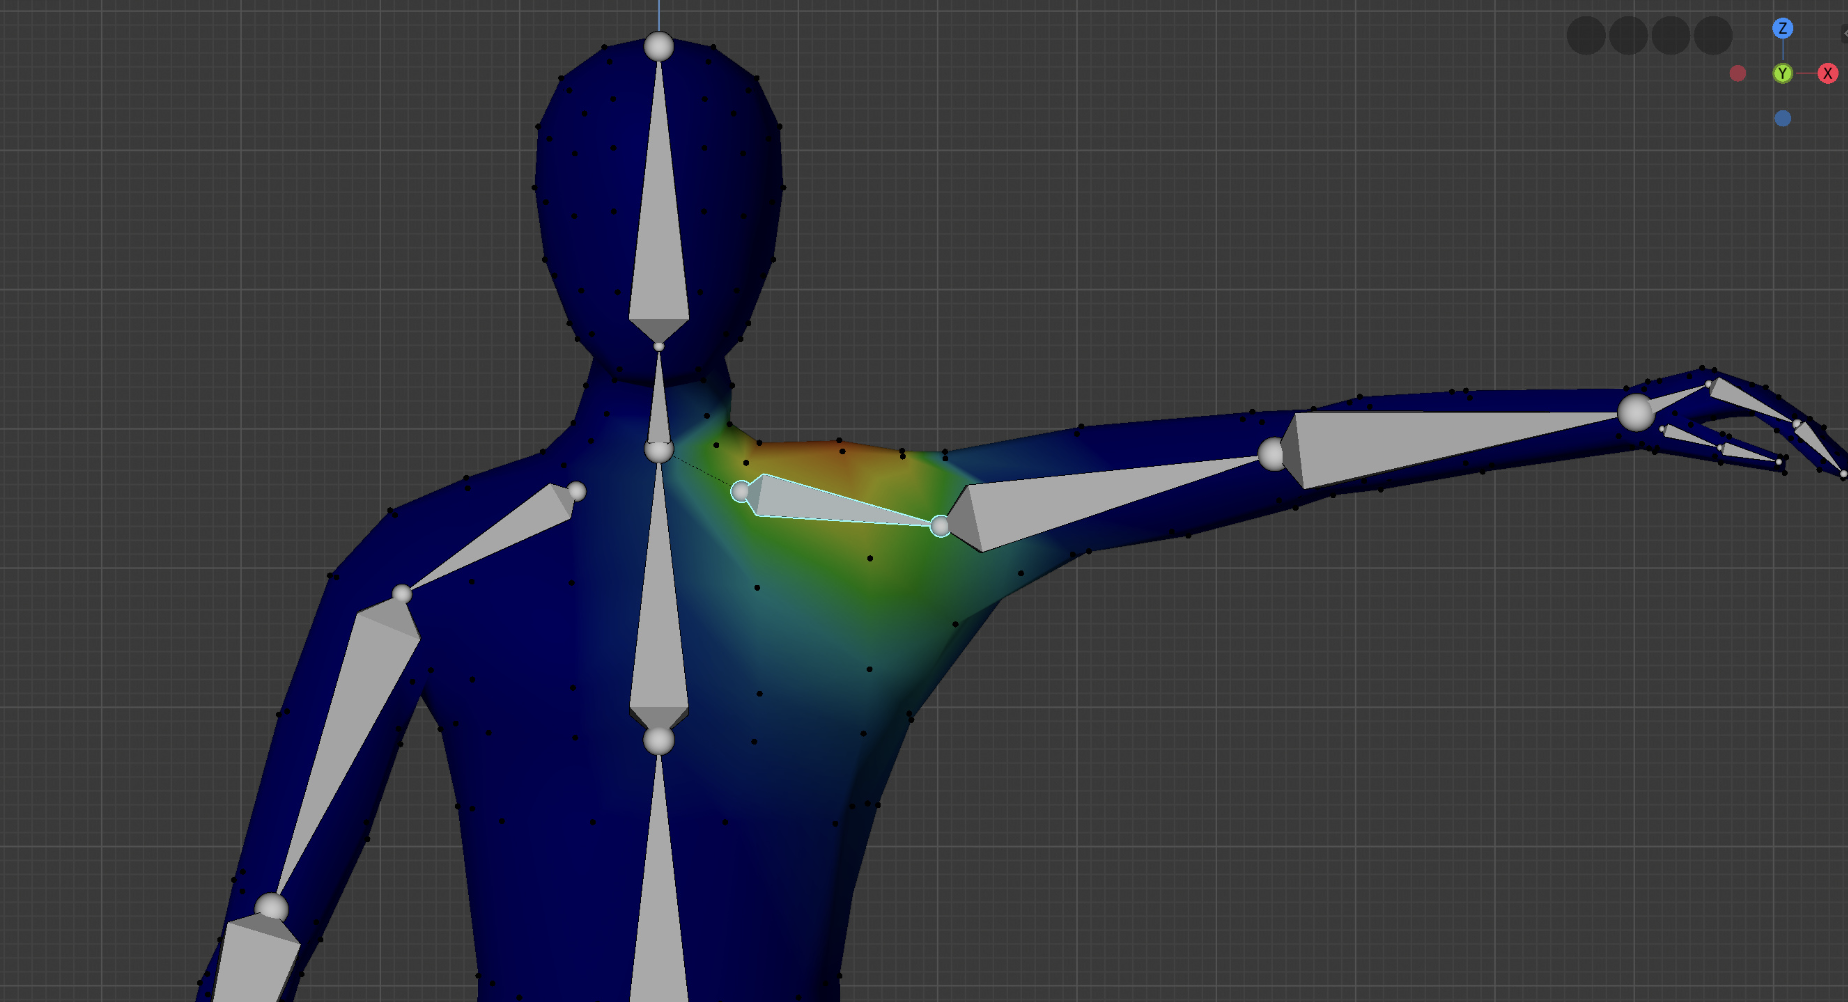
\includegraphics[width = 2.5in]{chapters/background_work/images/weight_painting.png} 
  \caption{Weight painting in Blender} 
  \label{fig:weight_painting} 
\end{figure}

\subsubsection{Rigging}
\label{ch:background_work:sign_language_synthesis:3d_techniques:rigging}

A rig is the final system used by the artists to animate the avatars. This is done by implementing all the above systems in order, i.e., creating a skeleton, mesh, texture, weight painting, facial blendshapes, implementing \gls{ik} and \gls{fk} systems, and adding constraints. Figure~\ref{fig:rig_example} shows an example of a rigged character, the "Rain rig" by Blender Studio.

\begin{figure} 
  \centering 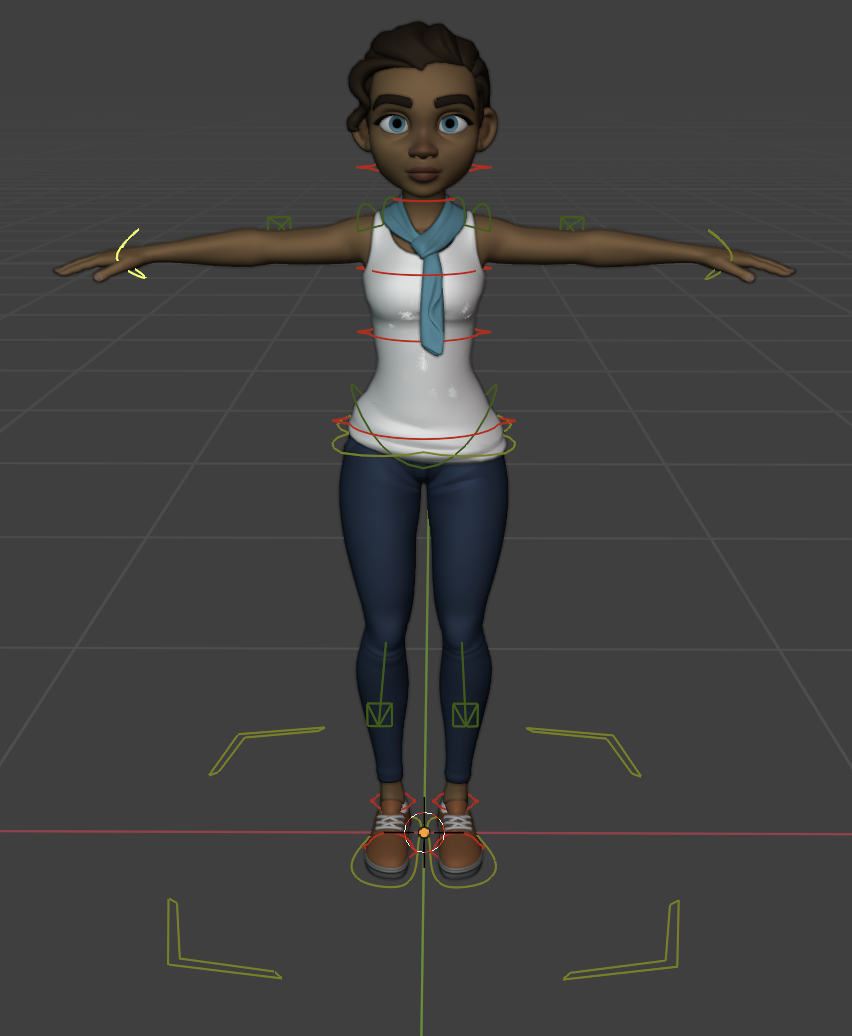
\includegraphics[width = 2.5in]{chapters/background_work/images/rig_example.png} 
  \caption{Rain rig by Blender studio} 
  \label{fig:rig_example} 
\end{figure}

\subsubsection{Procedural Avatar Creation}
\label{ch:background_work:sign_language_synthesis:3d_techniques:procedural_avatar_creation}

Procedural avatar creation involves the use of algorithms and software tools to automatically generate 3D characters with minimal manual intervention. This approach can significantly speed up the character creation process since it automates the creation of all of the avatar components discussed above. This allows rapid development of detailed and diverse avatars. This section explores several prominent tools and models used for procedural avatar creation.

\paragraph{MakeHuman}
\label{ch:background_work:sign_language_synthesis:3d_techniques:procedural_avatar_creation:makehuman}

MakeHuman is an open-source tool specifically designed for the rapid prototyping of humanoid avatars. It allows users to create 3D human models through an intuitive interface where parameters such as gender, age, ethnicity, and body proportions can be adjusted using sliders. Figure~\ref{fig:makehuman_example} demonstrates the process of creating an avatar using MakeHuman.

\begin{figure} 
  \centering 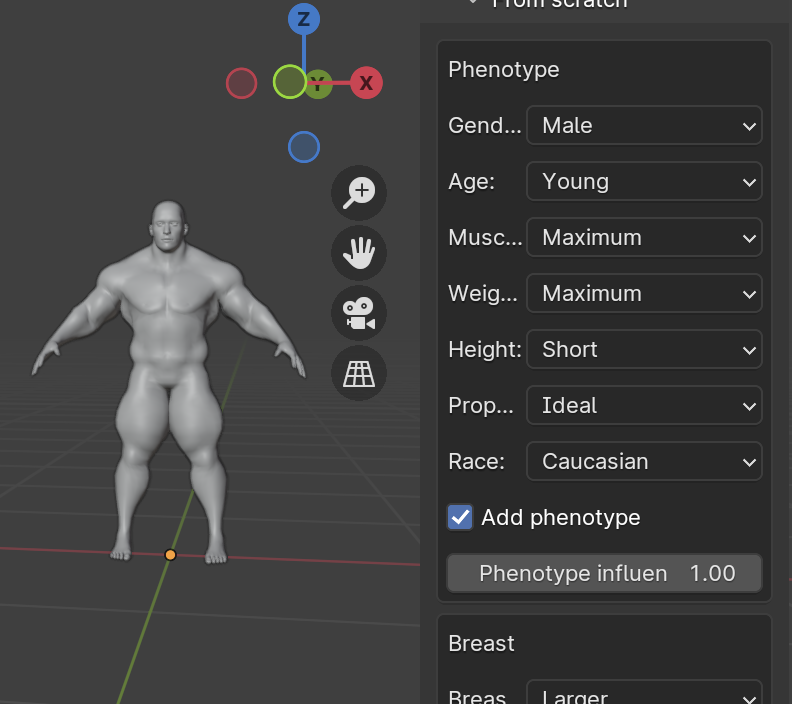
\includegraphics[width = 2.5in]{chapters/background_work/images/makehuman_example.png} 
  \caption{Avatar creation using MakeHuman} 
  \label{fig:makehuman_example} 
\end{figure}

\paragraph{SMPL-X or Meshcapade}
\label{ch:background_work:sign_language_synthesis:3d_techniques:procedural_avatar_creation:smpl_x_meshcapade}

Just like MakeHuman, SMPL-X can create avatars with parameters such as weight, height, age, etc. However, SMPL-X can also be created using images of a person. This allows it to be more realistic than MakeHuman. Figure~\ref{fig:smpl_creation_example} shows the process of creating an SMPL-X avatar using the Meshcapade tool.

\begin{figure} 
  \centering 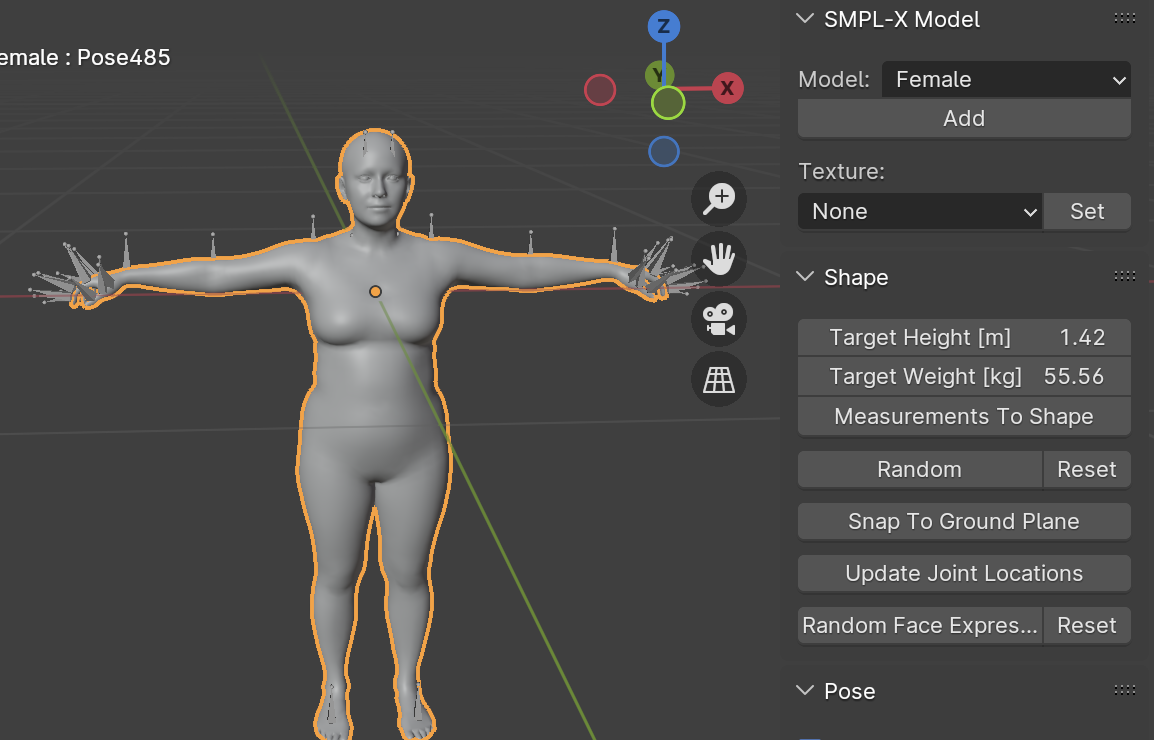
\includegraphics[width = 2.5in]{chapters/background_work/images/smpl_creation_example.png} 
  \caption{SMPL-X avatar creation using Meshcapade} 
  \label{fig:smpl_creation_example} 
\end{figure}

\paragraph{MetaHuman}
\label{ch:background_work:sign_language_synthesis:3d_techniques:procedural_avatar_creation:metahuman}

MetaHuman Creator (figure~\ref{fig:metahuman_example}), developed by Epic Games, is a tool for creating ultra-realistic digital humans. The tool's emphasis on realism and detail makes it a powerful resource for creating lifelike characters for games, films, and other interactive experiences. MetaHumans are the most realistic avatars available today, with high-quality textures, detailed facial expressions, and advanced animation controls.

\begin{figure} 
  \centering 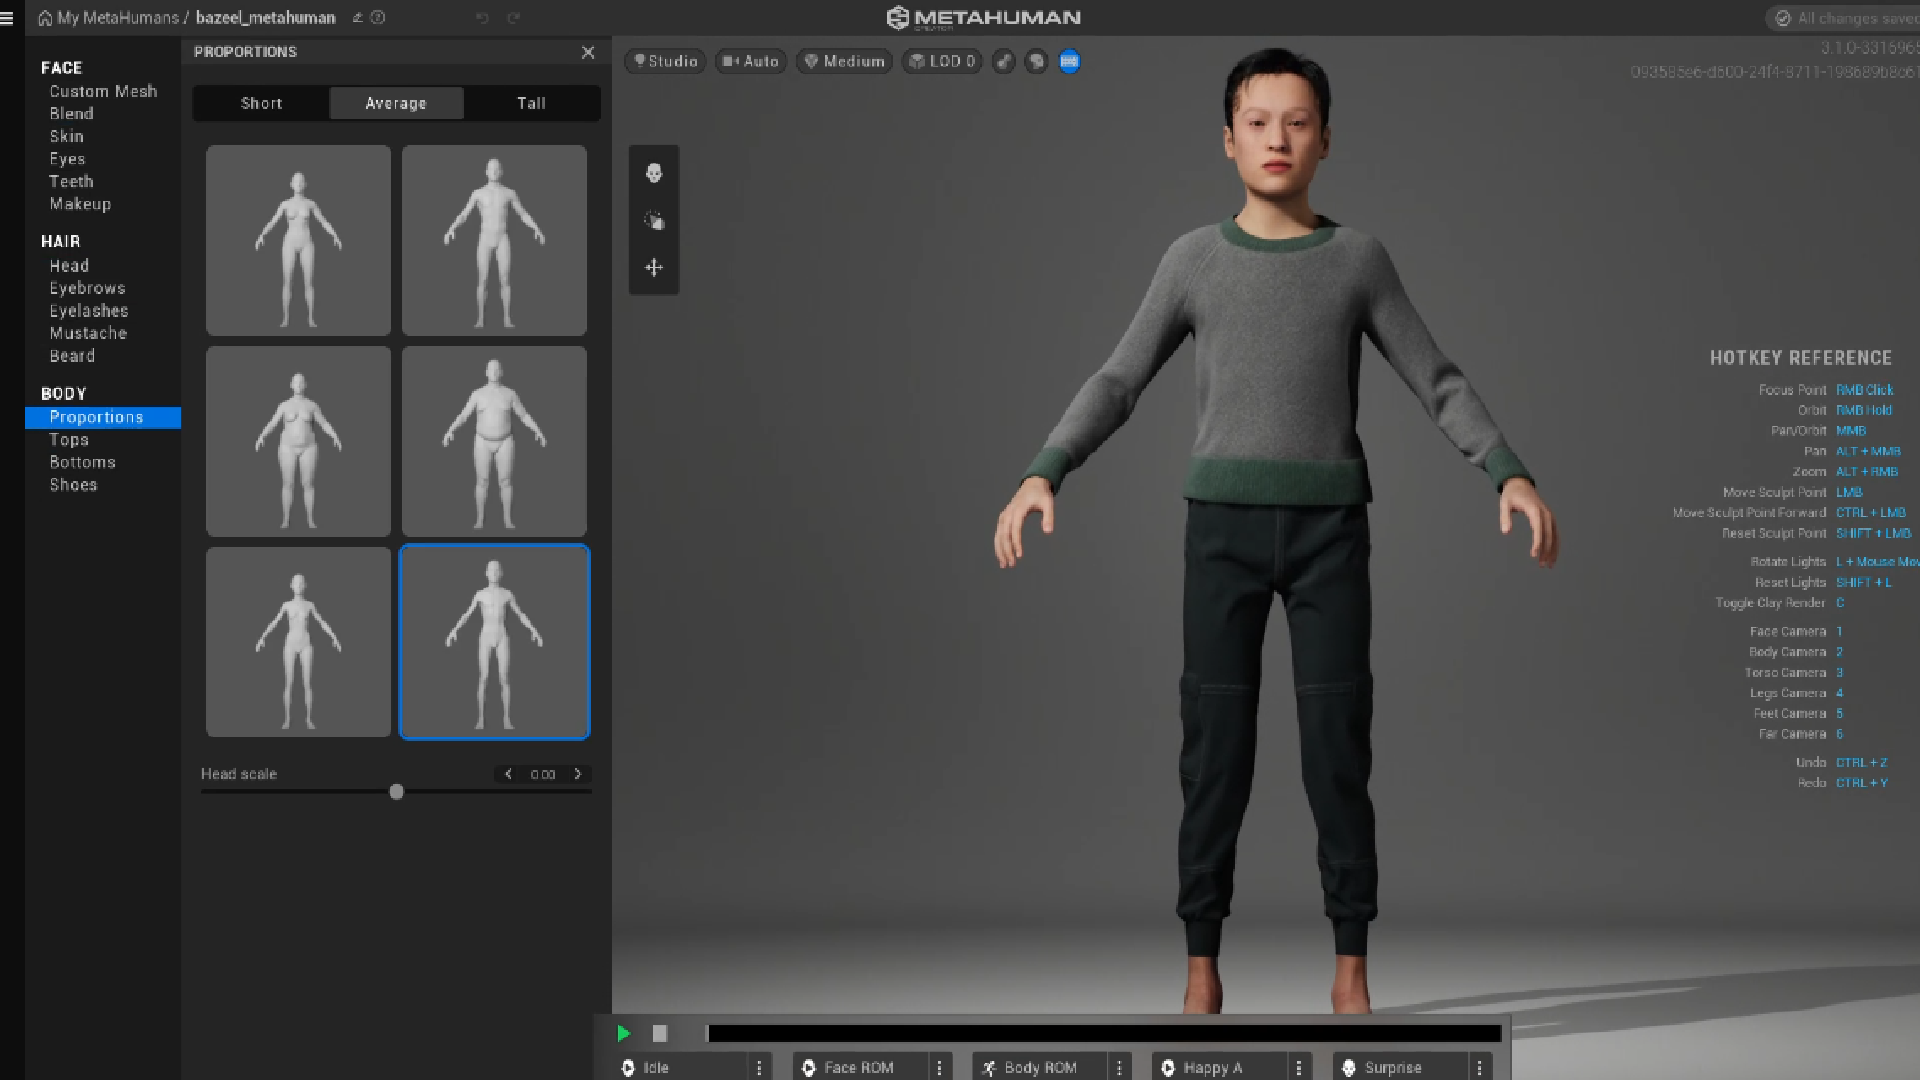
\includegraphics[width = 2.5in]{chapters/background_work/images/metahuman_example.png} 
  \caption{Avatar creation using MetaHuman} 
  \label{fig:metahuman_example}
\end{figure}

\subsubsection{Avatar Animation}
\label{ch:background_work:sign_language_synthesis:3d_techniques:avatar_animation}

The methods used for animating avatars range from manual to automated processes, each offering unique benefits and challenges. This section explores the key methods used in avatar animation.

\paragraph{Manual Keyframing}
\label{ch:background_work:sign_language_synthesis:3d_techniques:avatar_animation:manual_keyframing}

Manual keyframing is a traditional animation technique where animators define specific poses, known as keyframes, at critical points in time. These keyframes mark the start and end points of any smooth transition or movement. The intermediate poses are then calculated using interpolation. This method provides animators with precise control over every aspect of the avatar’s movement, making it ideal for achieving nuanced and detailed animations.

Figure~\ref{fig:keyframing} shows the process of manual keyframing to animate a sprite.

\begin{figure} 
  \centering 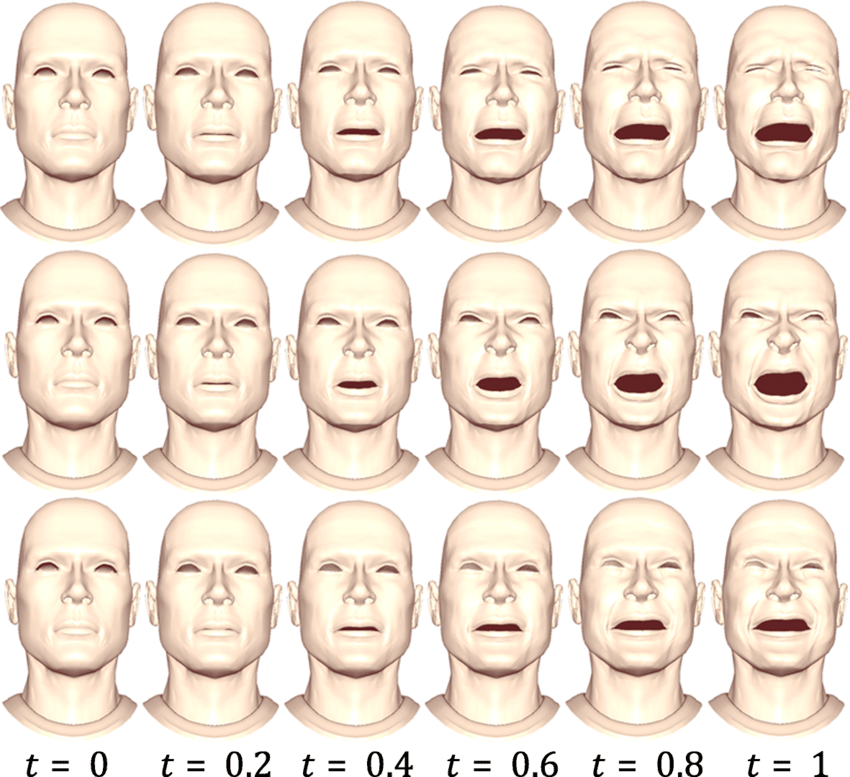
\includegraphics[width = 2.5in]{chapters/background_work/images/keyframing.png} 
  \caption{Manual keyframing to animate a sprite} 
  \label{fig:keyframing} 
\end{figure}

Along with keyframing, motion curves~\cite{10.1145/218380.218422} are used to control the interpolation between keyframes. These curves define the speed and timing of the animation, allowing animators to create smooth and natural movements. Common types of motion curves include linear, ease-in, ease-out, and bezier curves. By adjusting the shape and slope of these curves, animators can fine-tune the animation to achieve the desired effect. Figure~\ref{fig:motion_curves} shows examples of different motion curves used to fine-tune an animation.

\begin{figure} 
  \centering 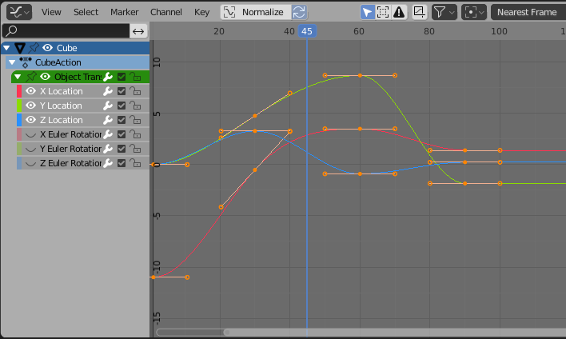
\includegraphics[width = 2.5in]{chapters/background_work/images/motion_curves.png} 
  \caption{Motion curves to finetune an animation} 
  \label{fig:motion_curves} 
\end{figure}

\paragraph{Mocap Retargeting}
\label{ch:background_work:sign_language_synthesis:3d_techniques:avatar_animation:mocap_retargeting}

Motion capture (mocap) retargeting involves capturing the movements of a real human actor and applying this data to a digital avatar. This process starts with recording an actor’s performance using a motion capture system, which tracks the actor’s movements through markers or sensors placed on their body. The recorded data is then mapped onto the avatar’s skeleton, a process known as retargeting. Mocap retargeting ensures highly realistic animations by directly transferring the nuances of human motion to the digital character. This technique is widely used in the entertainment industry, particularly in video games and films, to create lifelike animations.

Figure~\ref{fig:mocap} illustrates the process of motion capture and retargeting.

\begin{figure} 
  \centering 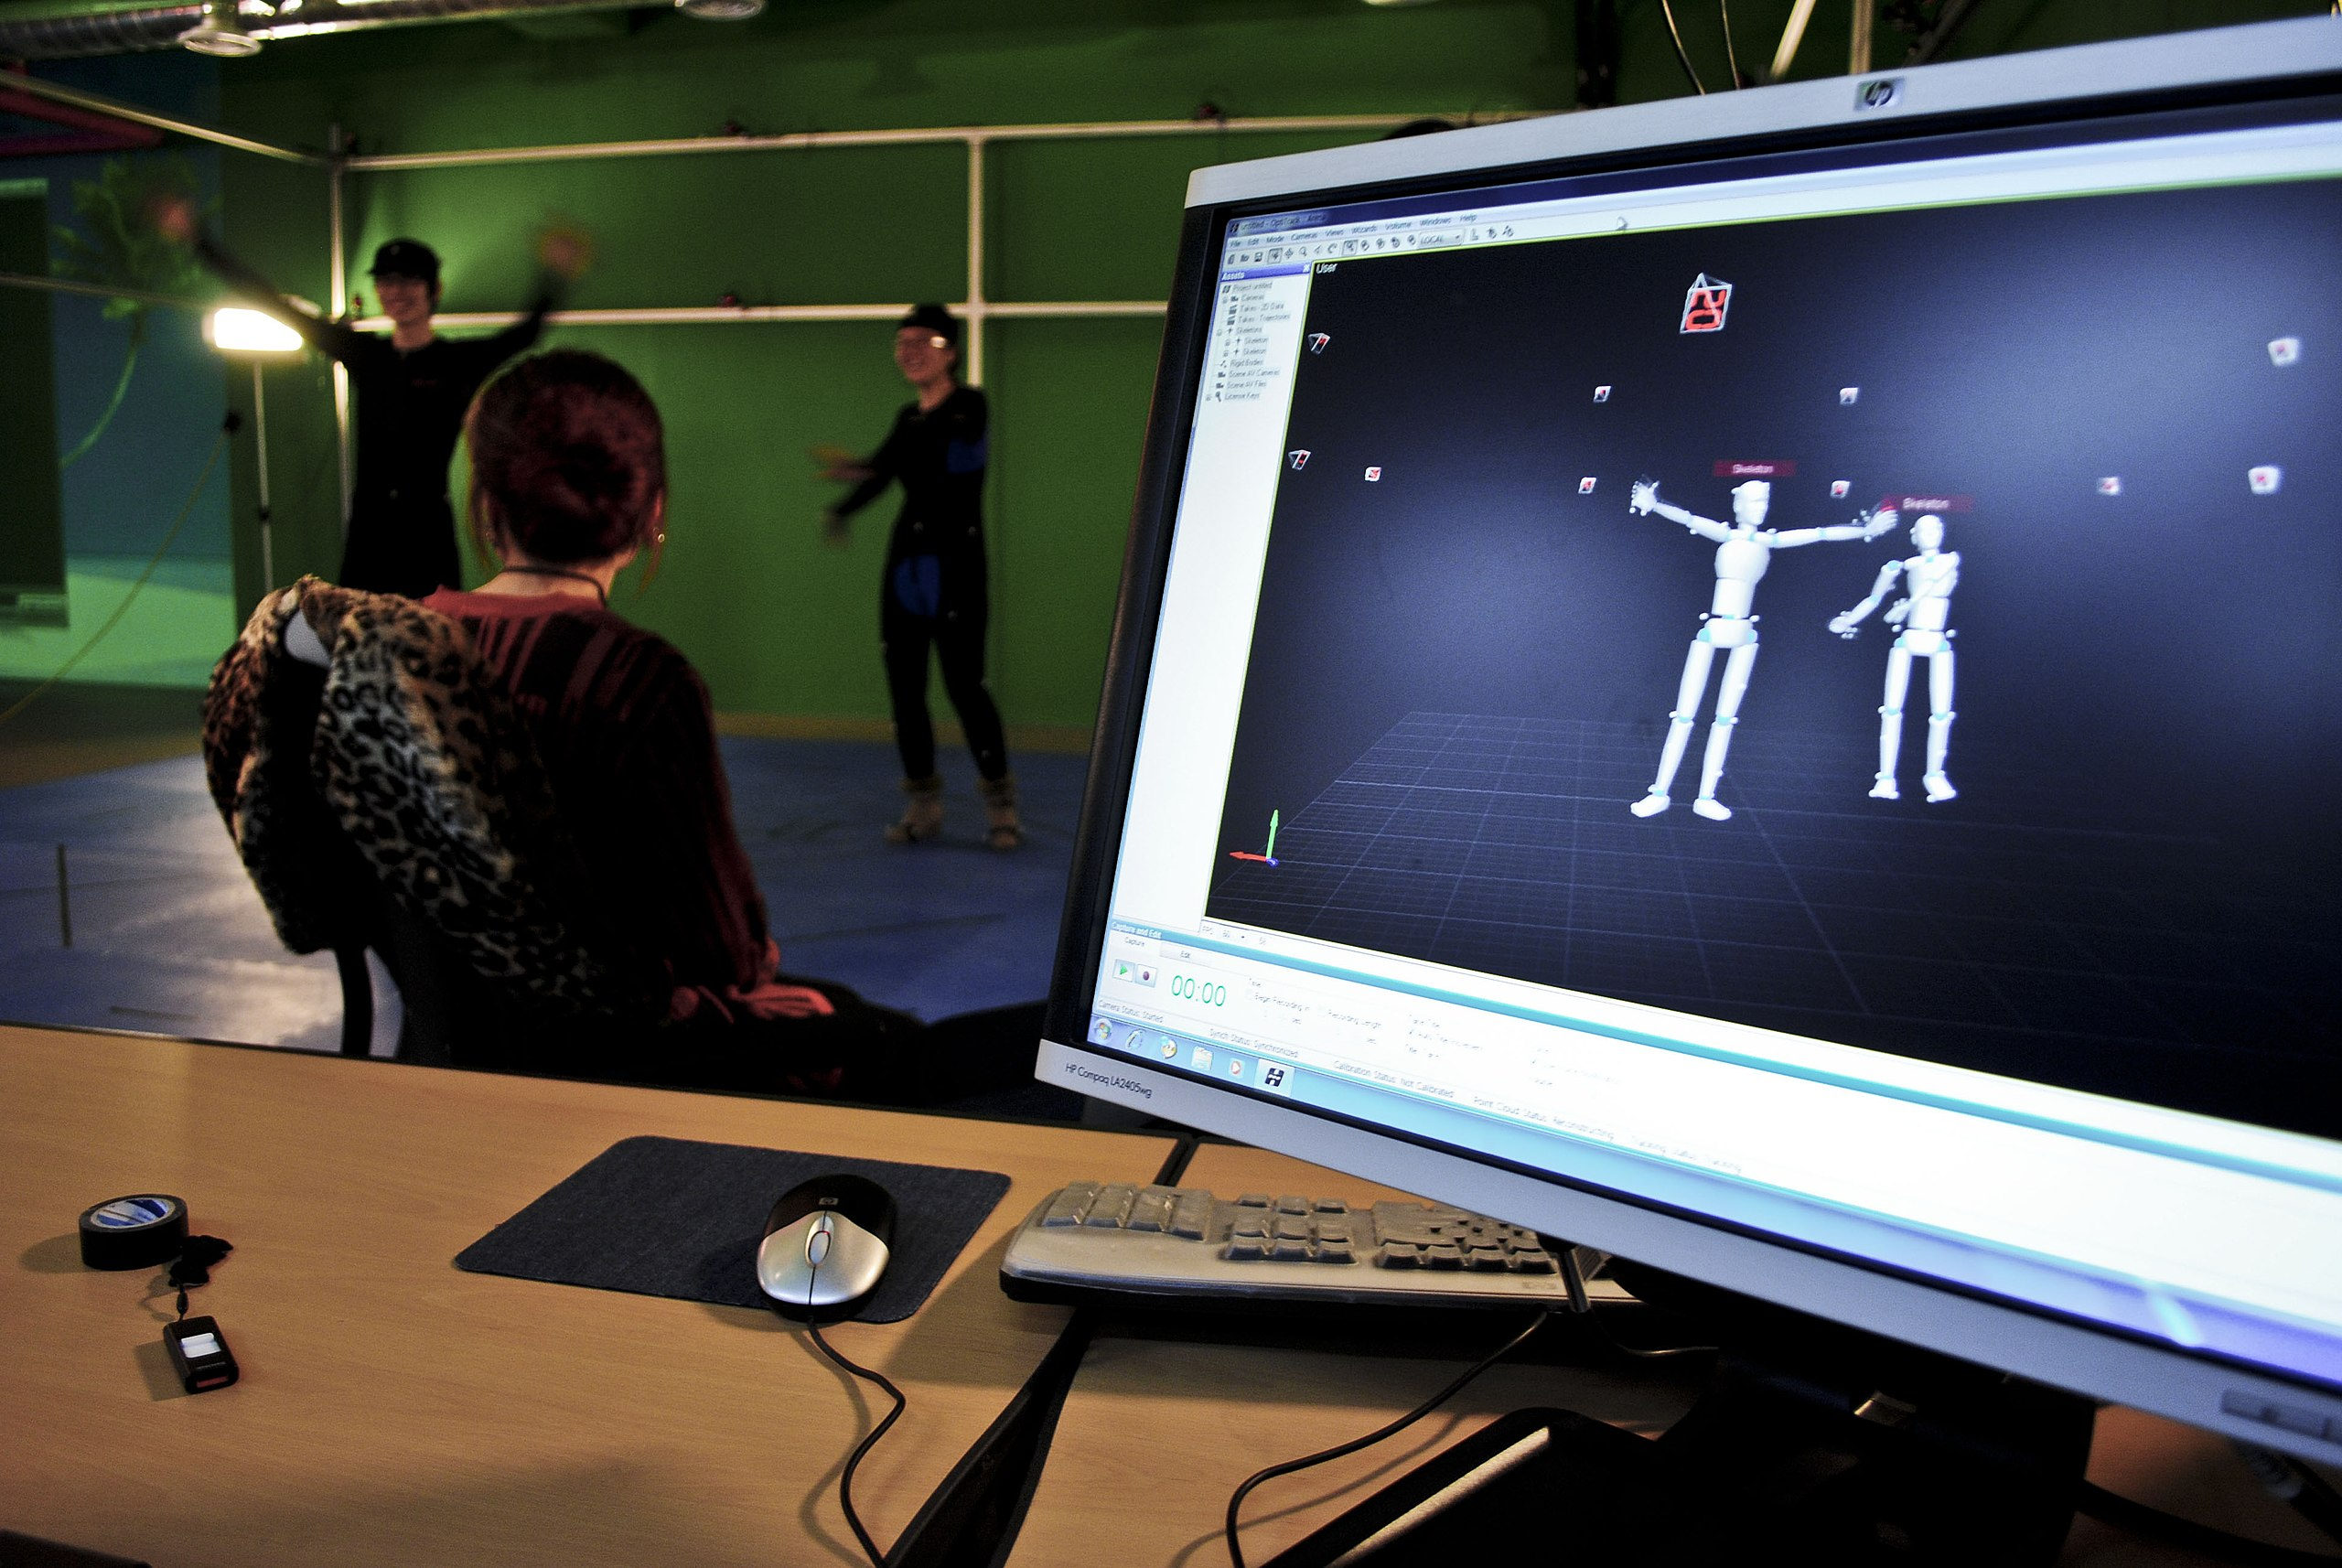
\includegraphics[width = 2.5in]{chapters/background_work/images/mocap.png} 
  \caption{Mocap capture and retargeting} 
  \label{fig:mocap} 
\end{figure}

Motion capture (mocap) retargeting offers a significant boost in animation speed and realism, but it does come with its challenges. It requires specialized equipment and involves intricate data processing, particularly when filtering out noise. Additionally, reusing mocap data across different avatars can be complex due to variations in body proportions and joint placements. Furthermore, segmenting mocap data into different parts for reuse can be difficult, limiting its flexibility in animation projects.

\paragraph{Kinematics}
\label{ch:background_work:sign_language_synthesis:3d_techniques:avatar_animation:kinematics}

Kinematics is used to define the motion of joints in a skeleton, allowing animators to create realistic and dynamic movements. Two key kinematic techniques used in avatar animation are \gls{fk} and \gls{ik}.

\subparagraph{\gls{fk}}
\label{ch:background_work:sign_language_synthesis:3d_techniques:avatar_animation:kinematics:forward_kinematics}

\gls{fk} is a method where the position and rotation of each joint in a skeleton are specified explicitly by the animator. This means that to move a hand, for example, the animator must adjust the shoulder, elbow, and wrist joints individually. \gls{fk} provides precise control over each joint, making it ideal for detailed and deliberate animations. However, it can be cumbersome for complex movements, as changes to one joint may require adjustments to multiple other joints to achieve a natural pose. Figure~\ref{fig:forward_kinematics_example} illustrates the forward kinematics process.

\begin{figure} 
  \centering 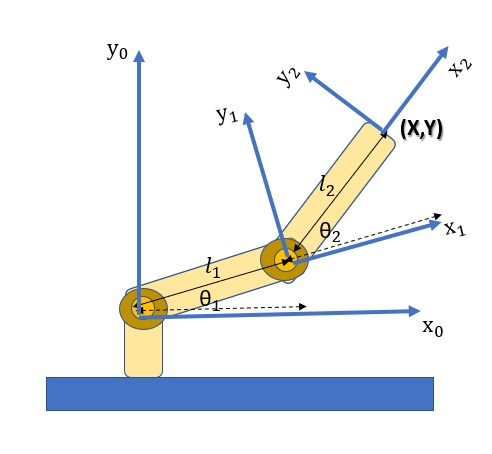
\includegraphics[width = 2.5in]{chapters/background_work/images/forward_kinematics_example.png} 
  \caption{FK} 
  \label{fig:forward_kinematics_example} 
\end{figure}

\subparagraph{\gls{ik}}
\label{ch:background_work:sign_language_synthesis:3d_techniques:avatar_animation:kinematics:inverse_kinematics}

\gls{ik} simplifies the animation process by allowing the animator to position the end effector (e.g., a palm or foot) directly (figure~\ref{fig:inverse_kinematics_example}). An \gls{ik} solver then computes the necessary joint rotations to achieve a desired position of the end effector. This technique is particularly useful for tasks like making a character’s hand reach a specific point or ensuring that feet remain planted on the ground. \gls{ik} is widely used in character animation to create natural and realistic movements more efficiently than \gls{fk}. \gls{ik} is popular area of research and there have been several ways to solve \gls{ik} problems.

\begin{figure} 
  \centering 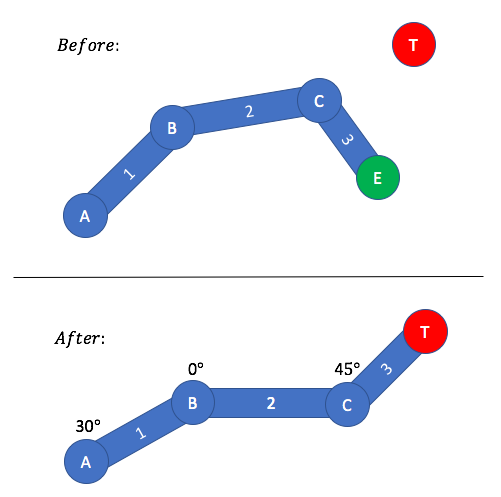
\includegraphics[width = 2.5in]{chapters/background_work/images/inverse_kinematics_example.png} 
  \caption{IK} 
  \label{fig:inverse_kinematics_example} 
\end{figure}

\begin{itemize} 
  \item \textbf{Jacobian-based methods}~\cite{4648032} solve the inverse kinematics (\gls{ik}) problem by linearizing the relationship between joint angles and end-effector positions through the calculation of the Jacobian matrix. These methods operate by formulating the \gls{ik} problem as a set of instantaneous task specifications, which are treated as constraints, such as positions, orientations, and other task-specific requirements. By iteratively adjusting joint angles to reduce the error between the current and target positions, they aim to minimize a cost function subject to multiple \gls{posture_constraint}s. Optimization techniques are employed to handle these constraints simultaneously, ensuring that the solution adheres to the defined task requirements. Despite their robustness in real-time applications, Jacobian-based methods can suffer from singularities, where solutions become unstable or unrealistic, as illustrated in Figure~\ref{fig:jacobian_based}.

  \item \textbf{\gls{ccd}}~\cite{kenwright2012inverse} simplifies the inverse kinematics (\gls{ik}) problem by adjusting one joint at a time to minimize the distance between the end-effector and the target position. It works by iteratively optimizing the position of each joint in the kinematic chain, starting from the end-effector and proceeding through each joint in sequence. This adjustment is done in a cyclic manner, where each joint is modified to ensure that the end-effector gets closer to the target while not significantly disrupting the previous adjustments. \gls{ccd} is computationally efficient and easy to implement, which makes it particularly popular in game engines. However, its greedy approach can lead to suboptimal solutions in more constrained or biomechanically complex setups, as illustrated in Figure~\ref{fig:ccdik}.

  \item \textbf{\gls{fabrik}}~\cite{aristidou2011fabrik} solves the inverse kinematics (\gls{ik}) problem through a two-phase iterative process: forward reaching and backward reaching. In the forward reaching phase, the algorithm starts from the base of the kinematic chain and moves towards the end-effector, adjusting joint positions to align with the target while respecting joint constraints. In the backward reaching phase, the process is reversed, starting from the end-effector and refining joint positions back toward the base to ensure convergence towards the target. Unlike other methods that focus on joint angles, \gls{fabrik} adjusts joint positions directly in two passes—from the end-effector to the root and back to the end-effector. This iterative process continues until the end-effector reaches the desired target within an acceptable tolerance. Known for its stability and simplicity, \gls{fabrik} is particularly effective in scenarios requiring natural joint configurations, as shown in Figure~\ref{fig:fabrik}.
\end{itemize}

\begin{figure}
    \centering 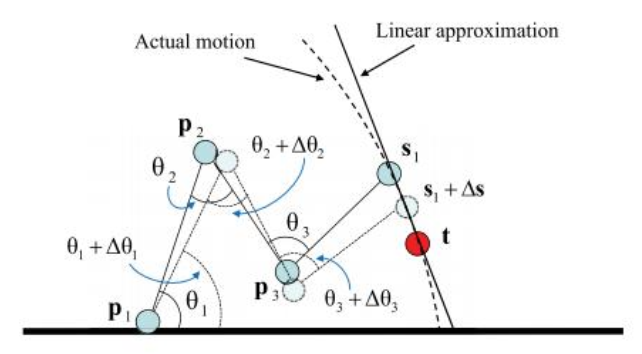
\includegraphics[width = 4in]{chapters/background_work/images/jacobian_based.png}
    \caption{Jacobian based IK solving (approximation of the first derivative)}
    \label{fig:jacobian_based}
\end{figure}

\begin{figure}
  \centering 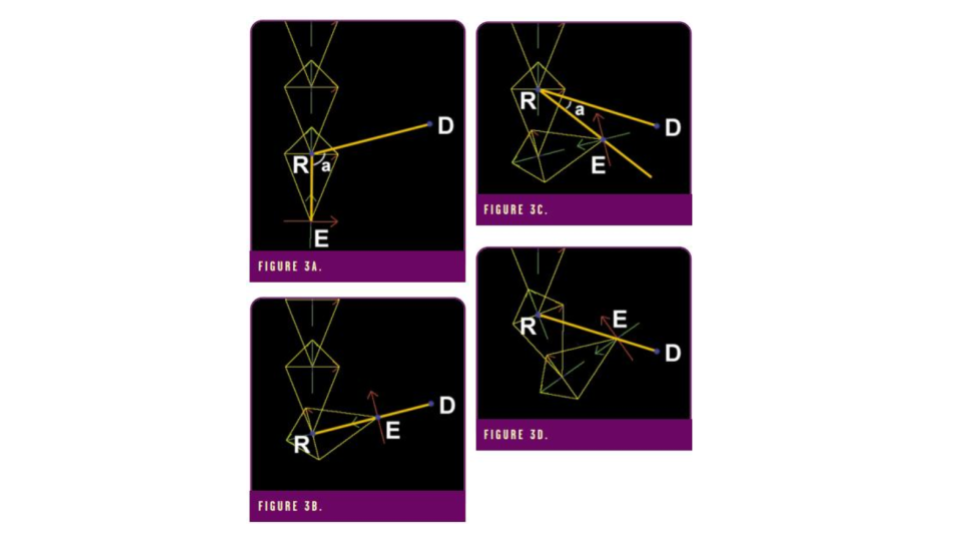
\includegraphics[width = 4in]{chapters/background_work/images/ccdik.png}
  \caption{Cyclic Coordinate Descent (CCD) IK solving (changes the rotation of a joint, one at a time)}
  \label{fig:ccdik}
\end{figure}

\begin{figure}
  \centering 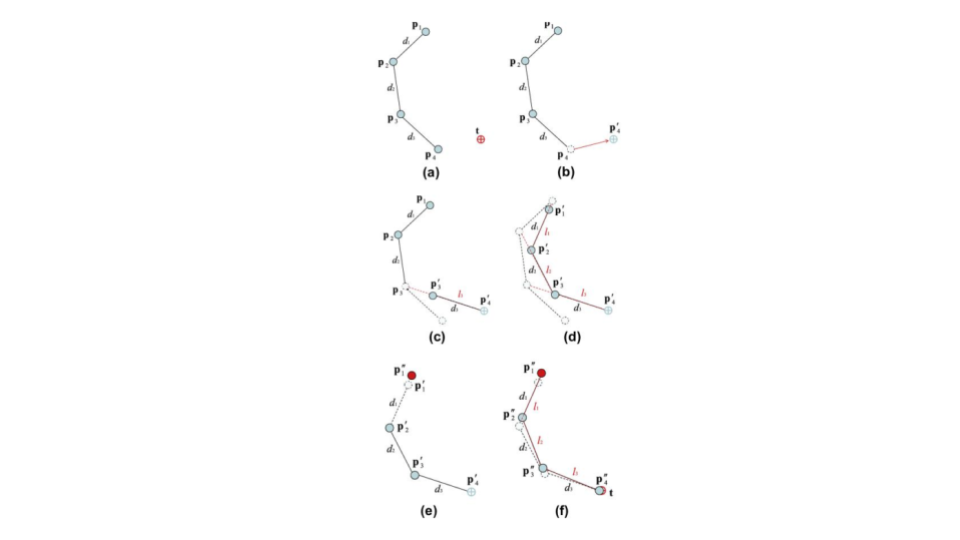
\includegraphics[width = 4in]{chapters/background_work/images/fabrik.png}
  \caption{FABRIK solving (updates coordinates in two passes)}
  \label{fig:fabrik}
\end{figure}

These classical \gls{ik} techniques, while computationally efficient, are prone to singularities, have limited support for complex joint constraints, and often result in unnatural or biomechanically unrealistic poses. As demonstrated in Figure~\ref{fig:problems_classical}, they struggle with overlapping chains and handling multiple end-effectors.

\begin{figure}
  \centering 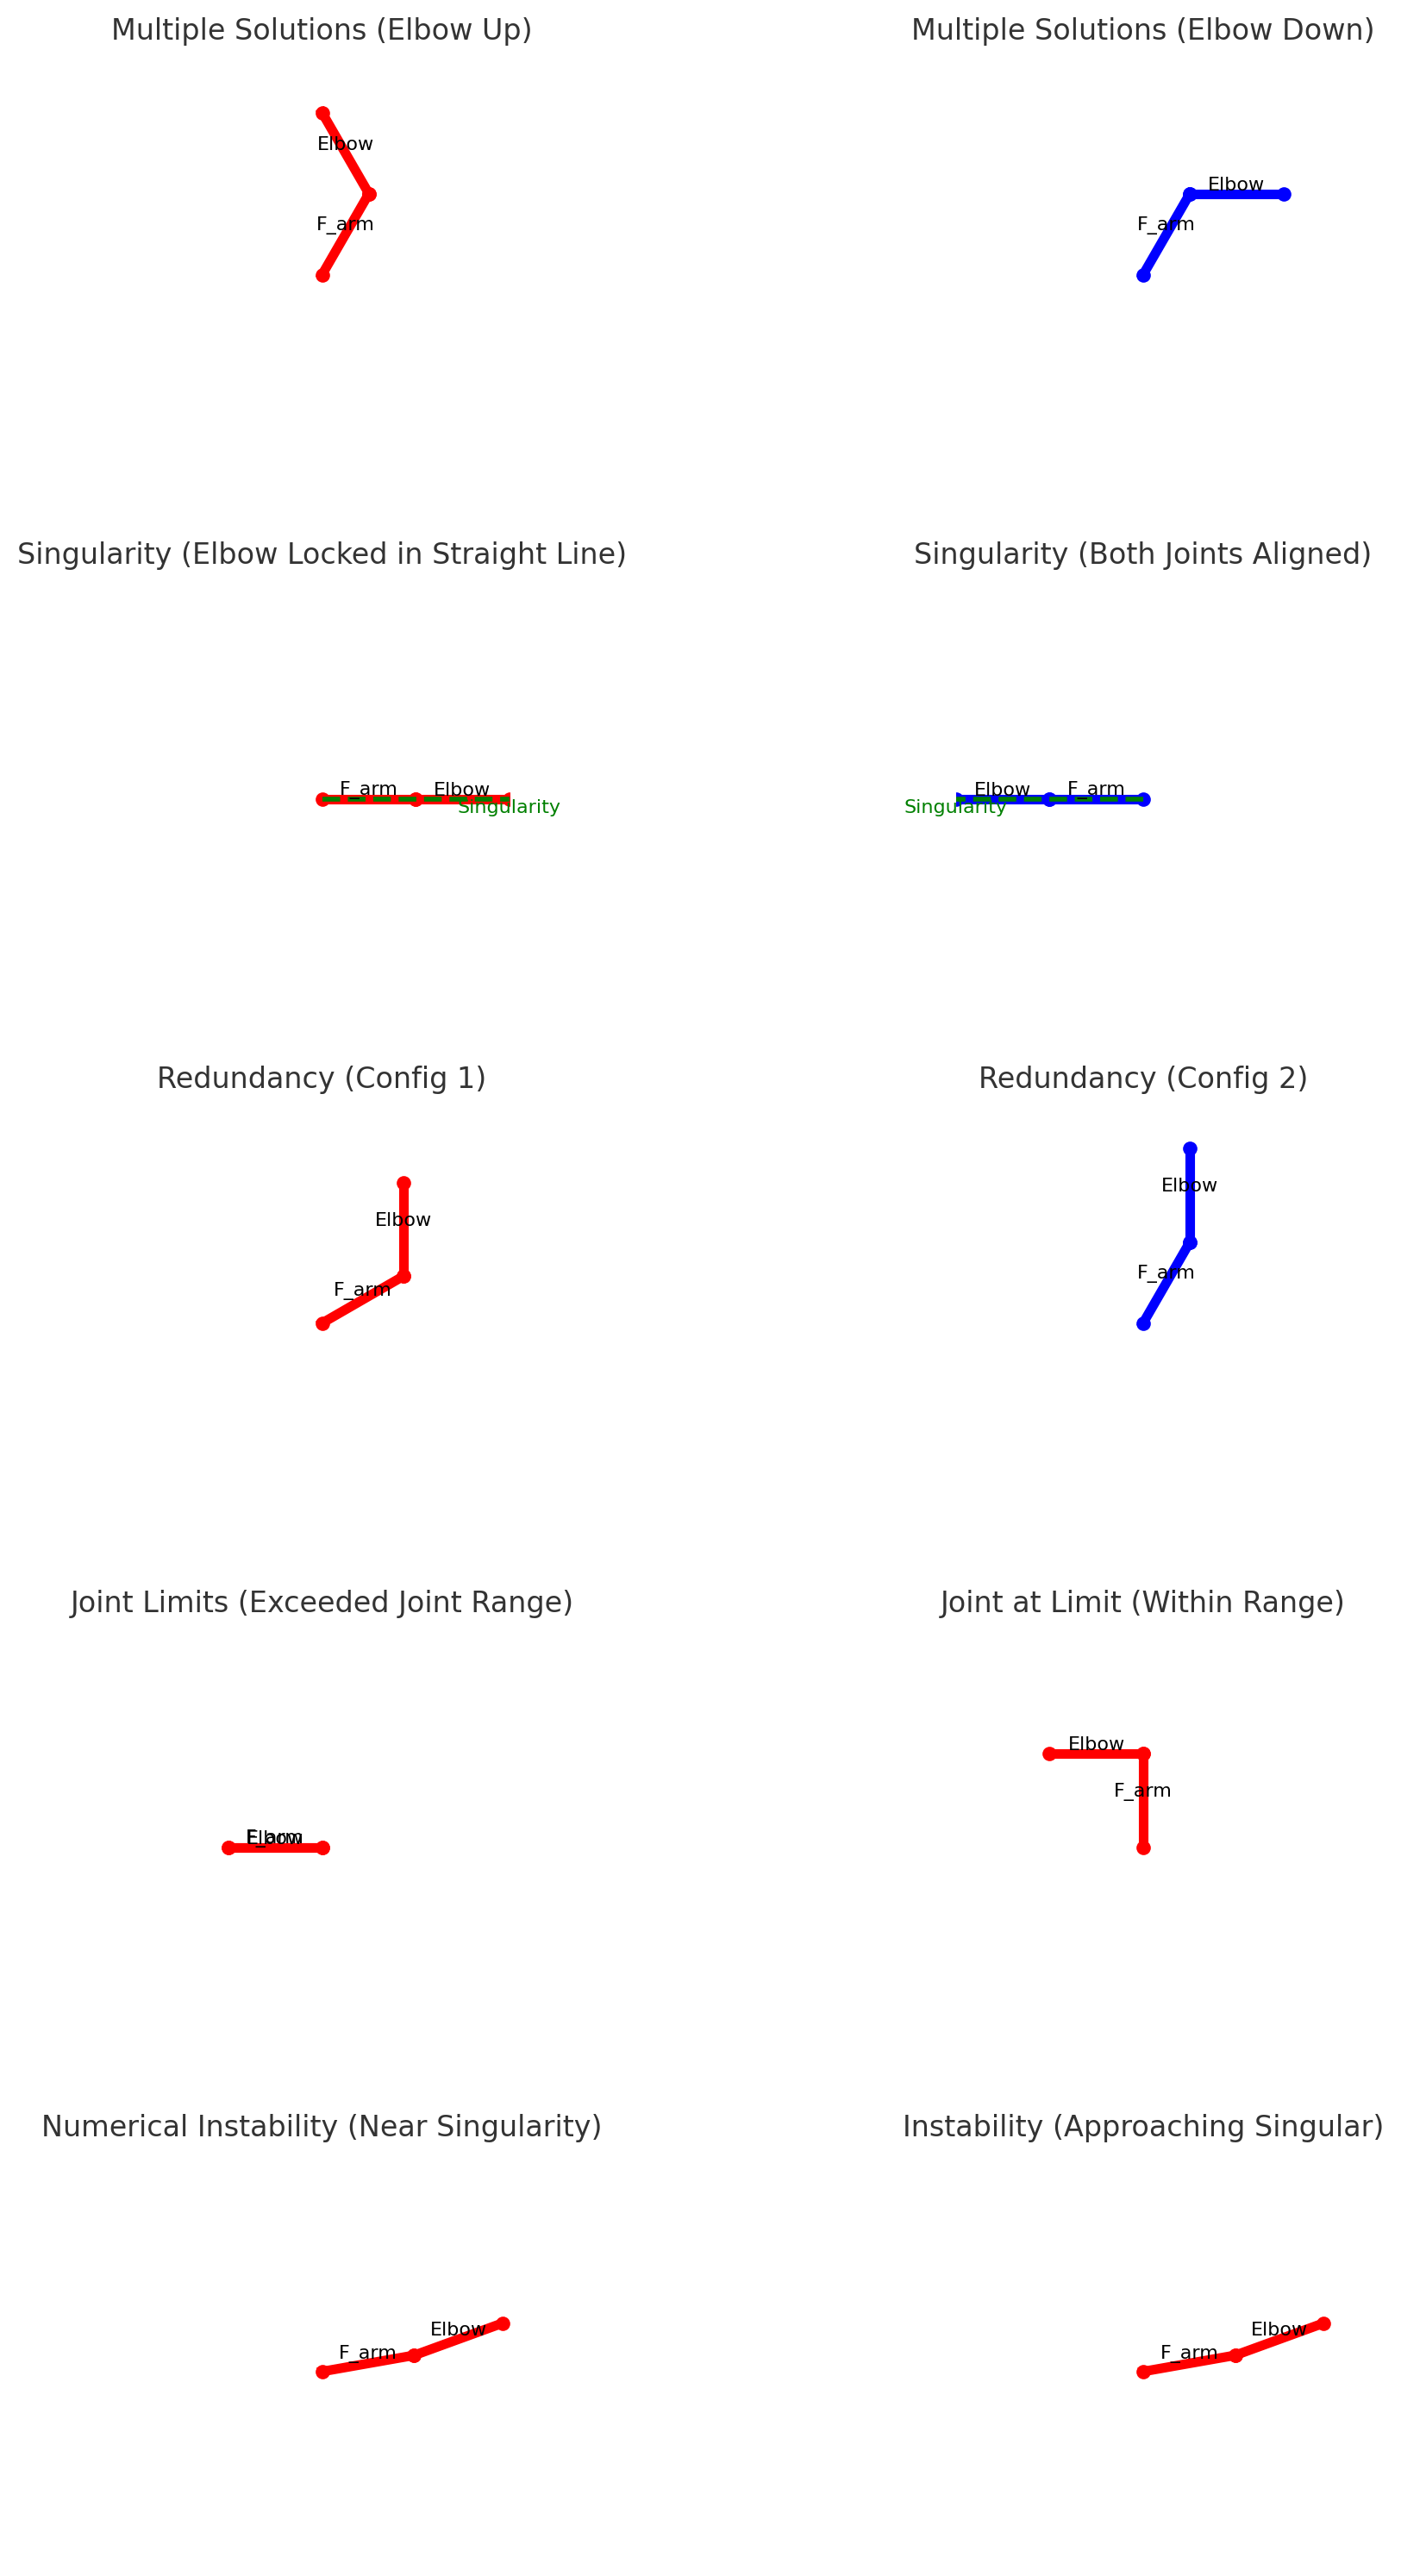
\includegraphics[width = 4in]{chapters/background_work/images/problems_classical.png}
  \caption{Problems with classical IK methods}
  \label{fig:problems_classical}
\end{figure}

\paragraph{Deep Learning and Character Animation}
\label{ch:background_work:sign_language_synthesis:3d_techniques:avatar_animation:deep_learning}

To address the shortcomings of classical kinematics methods, data-driven approaches have emerged, leveraging large datasets and machine learning to produce more flexible and realistic animations. This section explores some deep learning techniques used in character animation.

\subparagraph{Style-Based \gls{ik}}
\label{ch:background_work:sign_language_synthesis:3d_techniques:avatar_animation:deep_learning:style_ik}

Style \gls{ik}~\cite{grochow2004style} leverages machine learning to represent poses in a \gls{latent_space} using \gls{sgplvm}. By learning the distribution of poses, Style \gls{ik} generates stylized animations that adhere to aesthetic or functional constraints, making it especially useful in scenarios where mocap data is unavailable or infeasible. Figure~\ref{fig:style_ik} shows how poses are mapped in \gls{latent_space} for Style IK.

\begin{figure}
  \centering 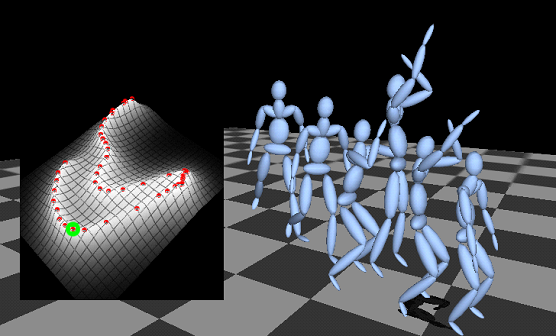
\includegraphics[width = 3in]{chapters/background_work/images/style_ik.png}
  \caption{Pose in latent space using Style IK}
  \label{fig:style_ik}
\end{figure}

\subparagraph{Motion Matching}
\label{ch:background_work:sign_language_synthesis:3d_techniques:avatar_animation:deep_learning:motion_matching}

Motion Matching represents a significant shift from traditional techniques by dynamically selecting the most appropriate animation from a large database of motion capture (mocap) data based on user inputs and contextual parameters. Ubisoft's \emph{For Honor} utilized this technique to create more fluid and responsive character animations, as shown in Figure~\ref{fig:for_honor}. Motion Matching's ability to break down animations into fine-grained clips allows for seamless transitions and natural movements.

\begin{figure}
  \centering 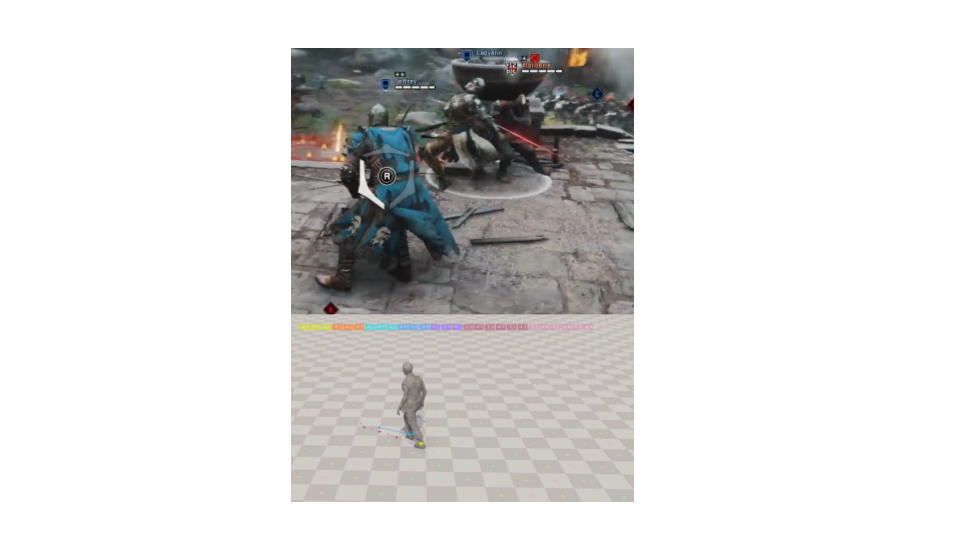
\includegraphics[width = 4in]{chapters/background_work/images/for_honor.png}
  \caption{Motion Matching in Ubisoft’s \emph{For Honor}}
  \label{fig:for_honor}
\end{figure}

\subparagraph{\gls{pfnn}}
\label{ch:background_work:sign_language_synthesis:3d_techniques:avatar_animation:deep_learning:pfnn}

\gls{pfnn}~\cite{10.1145/3072959.3073663} extends the principles of motion matching by incorporating phase information into the neural network’s weights, allowing the network to generate animations that align with the cyclical nature of bipedal movement (walking, running). Unlike traditional methods that blend animation clips, PFNN encodes the entire animation process within the neural network, providing more control and flexibility, as illustrated in Figure~\ref{fig:pfnn}.

\begin{figure}
  \centering 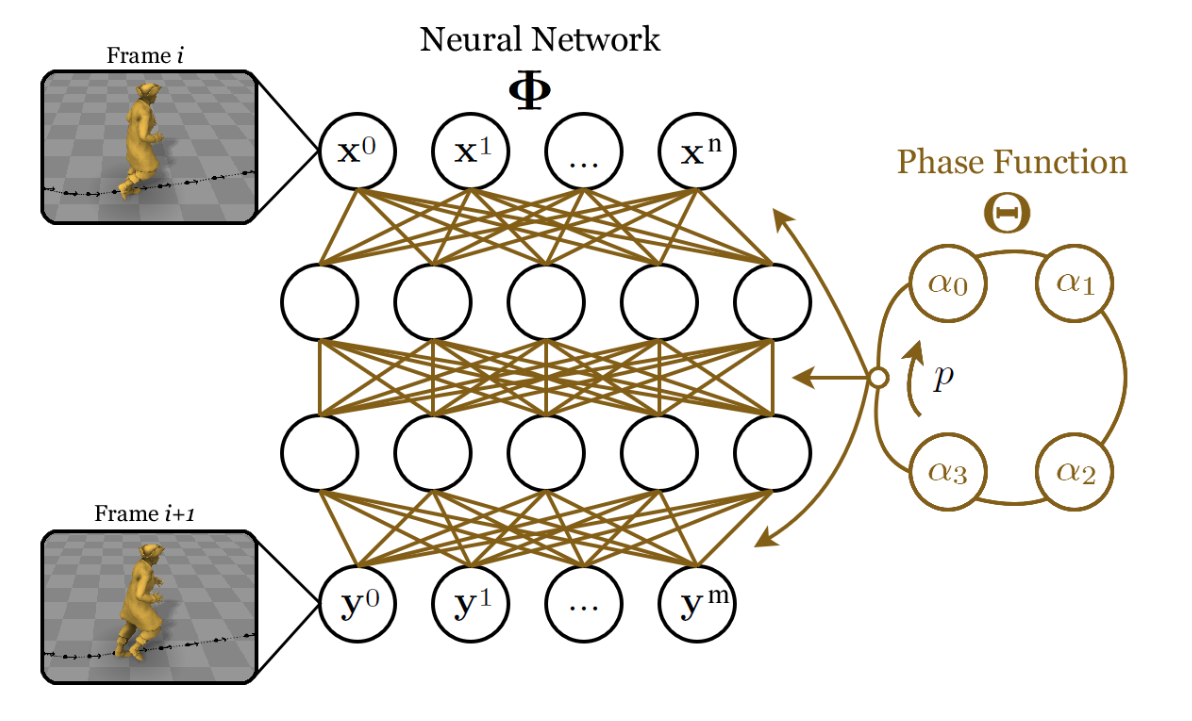
\includegraphics[width = 3in]{chapters/background_work/images/pfnn.png}
  \caption{Phase-Functioned Neural Networks (PFNN) for motion matching}
  \label{fig:pfnn}
\end{figure}

While these data-driven methods resolve many issues inherent to classical animation techniques, they bring challenges like the need for large amounts of training data and increased computational demands, particularly in real-time applications.

\subparagraph{Latent Space Representations for Pose Generation}
\label{ch:background_work:sign_language_synthesis:3d_techniques:avatar_animation:deep_learning:latent_space}

Latent space representations have become crucial in reducing the complexity of pose and motion data, allowing for more efficient and realistic pose generation and manipulation. VAEs~\cite{kingma2013auto}, such as those used in SMPLify-X~\cite{pavlakos2019expressive}, learn a probabilistic model of human poses. They can generate and manipulate poses in a lower-dimensional latent space, which can then be sampled to meet specific \gls{posture_constraint}s. SMPLify-X is particularly effective in estimating 3D poses from 2D images, as illustrated in Figure~\ref{fig:simplifyx}.

\begin{figure}
  \centering 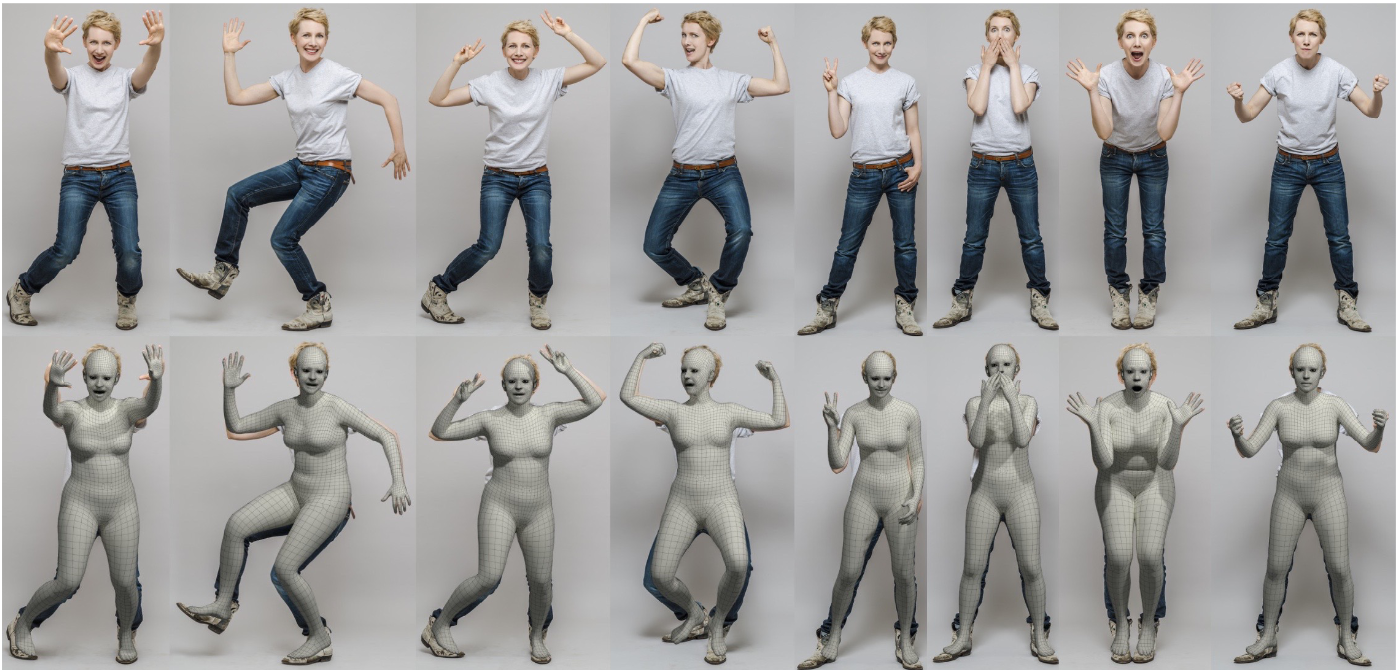
\includegraphics[width = 4in]{chapters/background_work/images/simplifyx.png}
  \caption{SMPLify-X generating poses from latent space}
  \label{fig:simplifyx}
\end{figure}

Pose manifolds~\cite{pavlakos2019expressive,tiwari2022pose, lu2023dposer} are pretty successful in creating a \gls{latent_space} representation of human poses. These manifolds are used to generate realistic and contextually appropriate poses by sampling from the learned distribution (a prior of human poses). This approach is particularly useful in generating diverse and expressive animations that adhere to specific constraints, such as bio-mechanical realism or stylistic preferences. Such pose manifolds can play a critical role by constraining pose generation to physically plausible configurations, as seen in figure~\ref{fig:pose_manifolds}.

\begin{figure}
  \centering 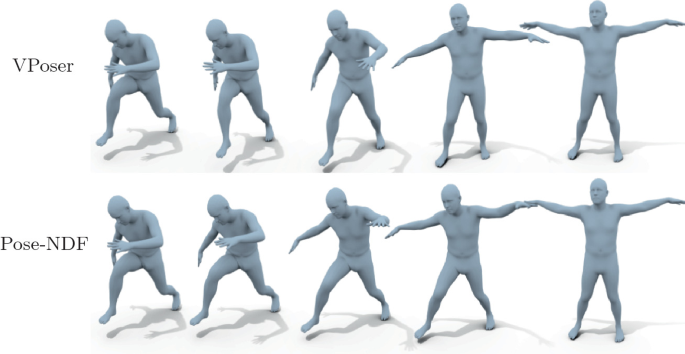
\includegraphics[width = 4in]{chapters/background_work/images/pose_manifolds.png}
  \caption{Pose regularization in a latent space}
  \label{fig:pose_manifolds}
\end{figure}

\paragraph{Representing Animation}
\label{ch:background_work:sign_language_synthesis:3d_techniques:avatar_animation:animation_timeline}

Animation timelines are often represented in the form of an animation timeline which provides visual representation of keyframes, motion curves, and other animation data. Animators use the timeline to organize and sequence animations, adjust timing and spacing, and fine-tune the overall motion of the avatar. Figure~\ref{fig:animation_timeline} shows an example of an animation timeline in Blender, a popular 3D animation software.

\begin{figure} 
  \centering 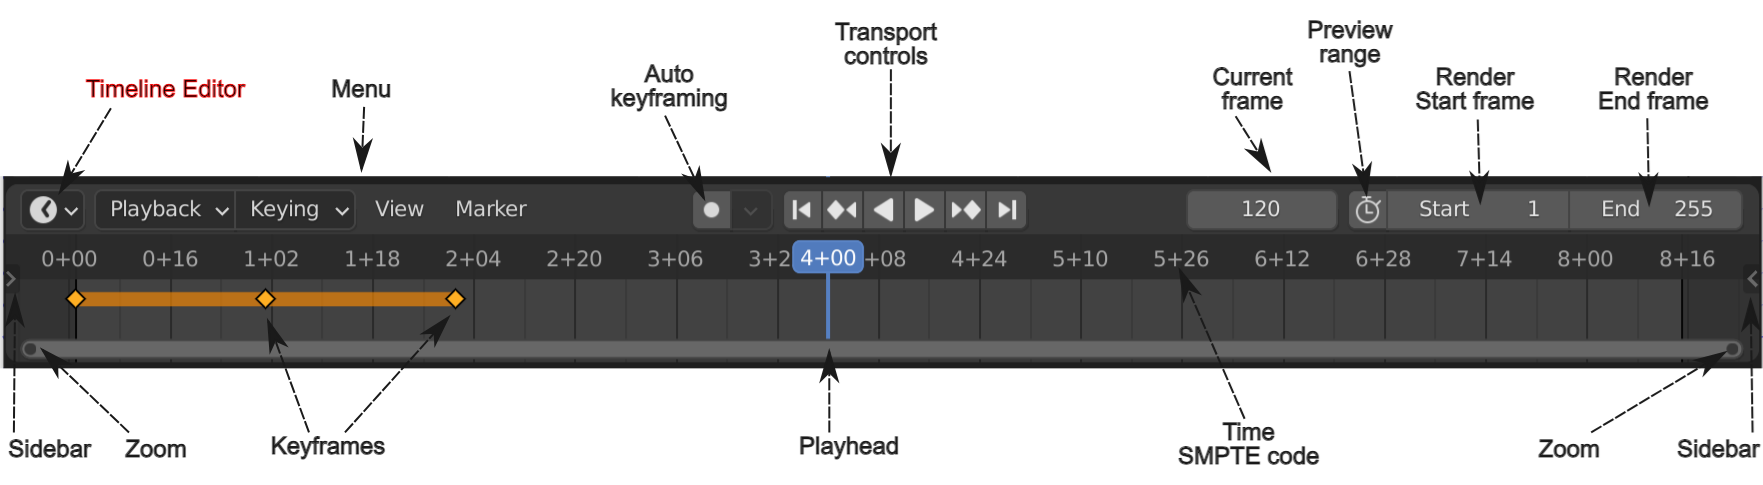
\includegraphics[width = 4in]{chapters/background_work/images/animation_timeline.png}
  \caption{Animation timeline in Blender} 
  \label{fig:animation_timeline}
\end{figure}

A multi-track timeline is a more advanced version of the animation timeline that allows animators to work with multiple tracks simultaneously. Multi-track interfaces are commonly used in video editing (figure~\ref{fig:video_edit}) and animation software to manage complex animations with multiple layers of motion data. Figure~\ref{fig:nle_editor} illustrates the \gls{nle} interface in blender, which represent the animation timeline in a multi-track format.

\begin{figure}
    \centering
    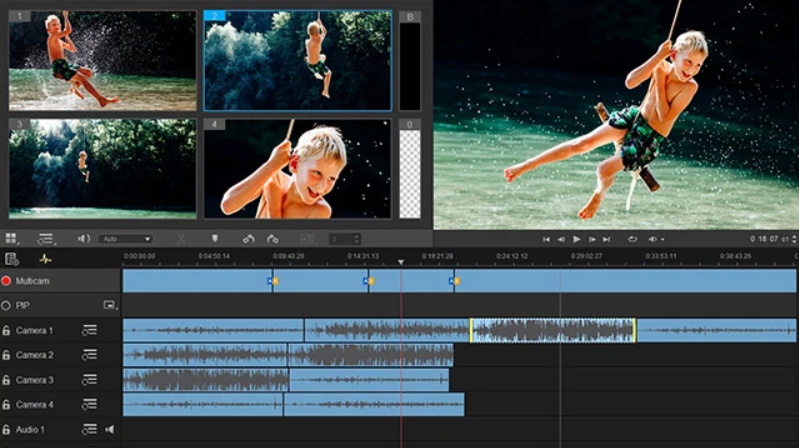
\includegraphics[width=0.8\textwidth]{chapters/background_work/images/video_editing.png}
    \caption{Video editing software interfaces with multiple tracks for editing video and audio clips.}
    \label{fig:video_edit}
\end{figure}

\begin{figure}
    \centering
    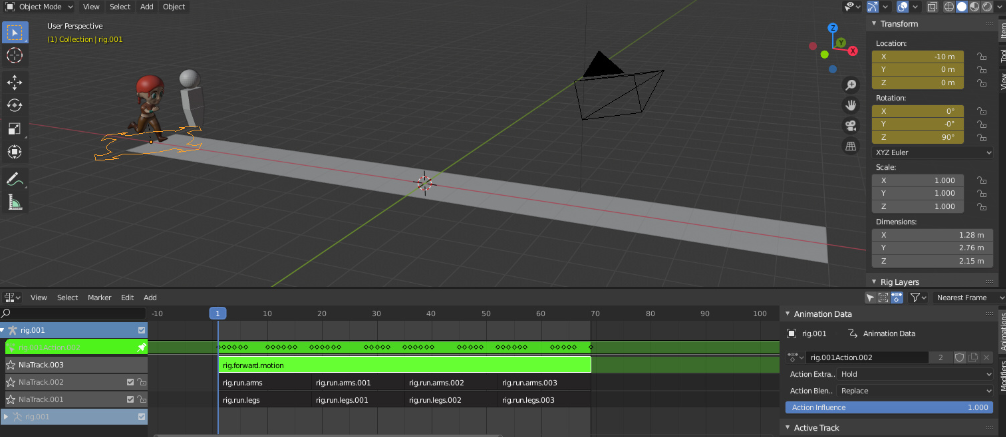
\includegraphics[width=0.8\textwidth]{chapters/background_work/images/nle_blender.png}
    \caption{Blender's NLE showing multiple tracks for editing animation clips.}
    \label{fig:nle_editor}
\end{figure}

Apart from artists, researchers too have recently explored multi-track timeline control for text-driven 3D human motion generation~\cite{petrovich24stmc}. The work introduces a novel way to address the limitations of previous methods that lacked fine-grained control over action composition and timing. This approach allows users to define multiple textual prompts within overlapping temporal intervals, enabling precise control over complex actions (figure~\ref{fig:multi_track_other}). The proposed Spatio-Temporal Motion Collage (STMC) method, which operates at test-time, integrates with pre-trained motion diffusion models to generate realistic motions that adhere to the specified timeline. However, it is not for use in \gls{sl} synthesis, where precise and context-sensitive hand and body gestures are required, as it relies heavily on models not specifically designed for such detailed tasks.

\begin{figure}
    \centering
    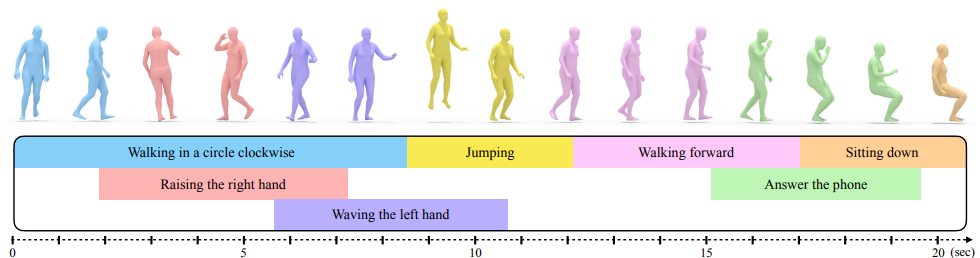
\includegraphics[width=0.9\textwidth]{chapters/background_work/images/multi_track_other.png}
    \caption{Multi-track timeline control for text-driven 3D human motion generation.}
    \label{fig:multi_track_other}
\end{figure}

In the context of \gls{sl} synthesis, a multi-track timeline is used by Paula~\cite{filhol2017synthesizing} (more discussed in section~\ref{ch:background_work:sign_language_synthesis:3d_techniques:sign_language_synthesis_systems:azee_based:paula}), a system that uses pre-recorded motion data to generate multi-track animations using AZee. Paula's interface is tailored for creating \gls{sl} content, with each track representing a different aspect of the \gls{sl}. Figure~\ref{fig:paula} shows the Paula interface with a multi-track timeline for \gls{sl} synthesis.

\begin{figure}[h]
    \centering
    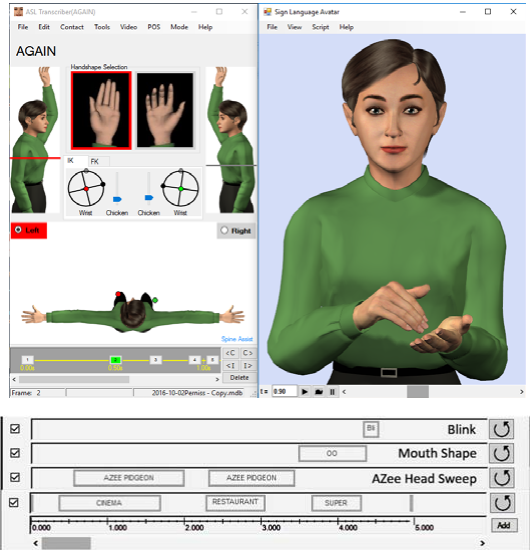
\includegraphics[width=0.8\textwidth]{chapters/background_work/images/paula_multi_track.png}
    \caption{Paula interface showing a multi-track timeline for SL synthesis.}
    \label{fig:paula}
\end{figure}

\paragraph{Motion Curves}
\label{ch:background_work:sign_language_synthesis:3d_techniques:avatar_animation:motion_curves}

Motion curves, have been extensively used in 3D character animation to control the timing and spacing of movements. These curves provide a graphical representation of a parameter's change over time, making them an essential tool in achieving realistic and fluid motion in animations(figure~\ref{fig:fcurves_blender}). Early foundational work by Witkin and Kass~\cite{witkin1988spacetime} introduced spacetime constraints, which used optimization techniques to control motion curves in generating realistic animations under physical constraints. This idea has evolved, and modern techniques now integrate deep learning models with motion curves to enhance control and automate the generation of complex animations. This is particularly useful in applications like motion inbetweening, where interpolating between keyframes requires precise control over motion curves to ensure smooth transitions and realistic movements (figure~\ref{fig:inbetweening_transformers})~\cite{10.1145/3550454.3555454}. However, traditional mathematical optimization techniques are still widely in use. For example use of tangent-space optimization~~\cite{10.1145/3306346.3322938} to control character interpolations by allowing animators to directly manipulate positions and orientations of the posture by manipulating the tangent of the curve. This minimizes the need for additional keyframes. It also ensures smooth transitions while respecting \gls{posture_constraint}s like joint limits and contact points, integrating seamlessly into existing animation workflows (figure~\ref{fig:inbetweening_disney}). 

\begin{figure}
    \centering 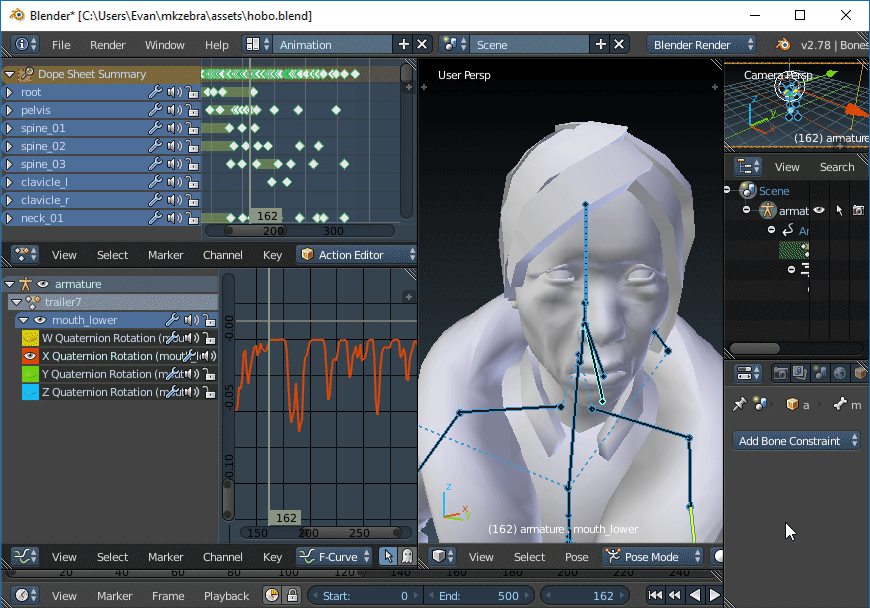
\includegraphics[width = 2.5in]{chapters/background_work/images/fcurves_blender.png}
    \caption{F-curves in Blender}
    \label{fig:fcurves_blender}
\end{figure}

\begin{figure}
    \centering 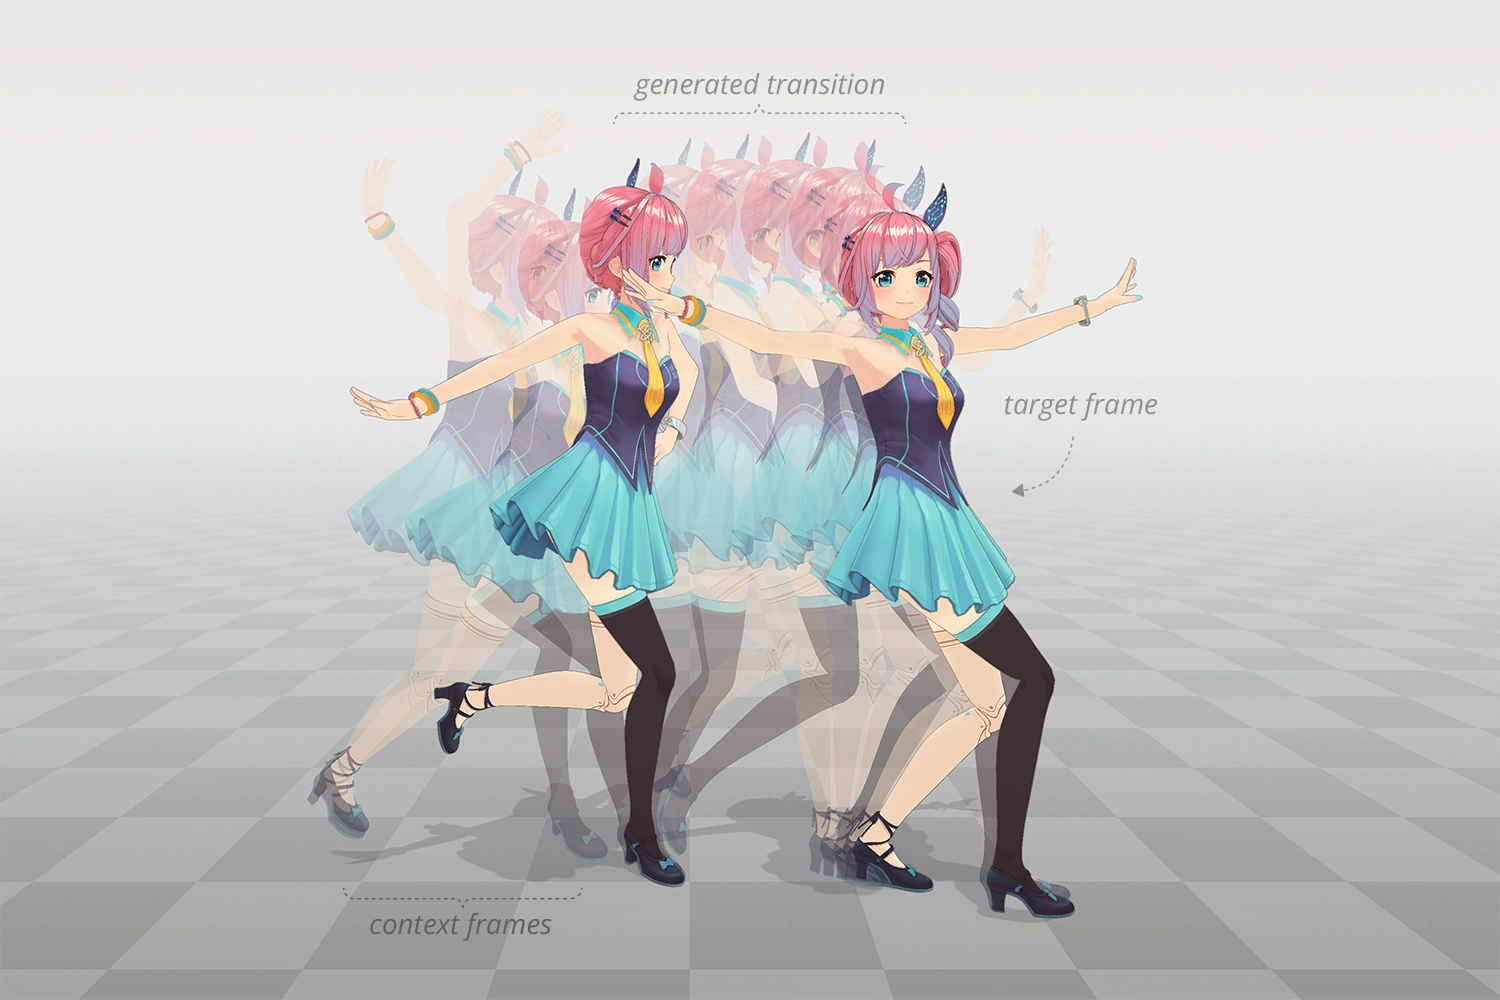
\includegraphics[width = 2.5in]{chapters/background_work/images/inbetweening_transformers.jpg}
    \caption{Motion Inbetweening using 2 stage Transformers~\cite{10.1145/3306346.3322938}}
    \label{fig:inbetweening_transformers}
\end{figure}

\begin{figure}
    \centering 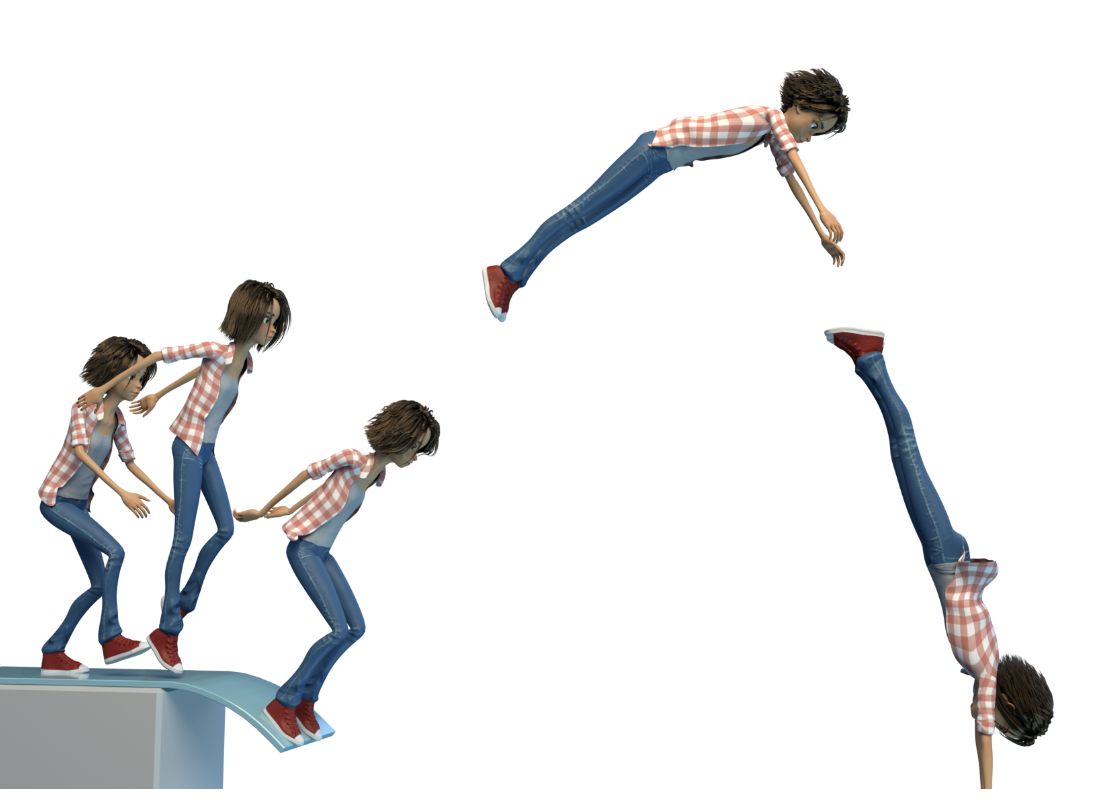
\includegraphics[width = 2.5in]{chapters/background_work/images/inbetweening_disney.png}
    \caption{Tangent-Space Optimization use to create dive animation}
    \label{fig:inbetweening_disney}
\end{figure}

In the context of \gls{sl} synthesis, SIGN MOTION~\cite{inproceedings} discuss the use of 3D motion analysis to accurately capture and animate \gls{sl} gestures by extracting motion curve parameters from sensors like Microsoft Kinect. These motion curves, which represent the trajectories of movements made during signing, are essential for animating virtual signers in a natural and precise manner. The paper highlights how these curves are mathematically defined, including their type, plane of motion, and velocity, which are then used to recreate realistic \gls{sl} animations, enhancing applications like \gls{sl} recognition and machine translation.

\paragraph{Motion Templates}
\label{ch:background_work:sign_language_synthesis:3d_techniques:avatar_animation:motion_templates}

Motion templates offer a reusable framework for applying pre-defined motion patterns across different characters or scenarios. These templates are essentially built upon motion curves that define the motion's parameters, allowing for efficient replication and adaptation of complex motions. The concept of motion templates has been widely adopted in various fields, from character animation to robotic motion planning. Modern approaches often combine motion templates with machine learning techniques to facilitate the adaptation of these templates to new contexts, such as different character anatomies or environmental conditions.

In the context of character animation, motion templates can be particularly advantageous. The reusable nature of these templates allows for the consistent production of motion across different avatars while ensuring that the nuances of each motion are preserved. A method for controlling avatars using clustered motion segments from a large motion capture database was introduced by~\cite{10.1145/566654.566607}, enabling efficient real-time animation with an intuitive user interfaces.

\paragraph{Procedural Animation}
\label{ch:background_work:sign_language_synthesis:3d_techniques:avatar_animation:procedural_animation}

Procedural animation techniques use algorithms and rules to generate motion automatically, rather than relying on manual keyframing or motion capture data. These techniques are particularly useful for creating dynamic and responsive animations that adapt to changing conditions or user interactions. Procedural animation can be applied to various aspects of avatar animation, including locomotion, facial expressions, and secondary motion.

\subparagraph{Data-Driven Constraint-Based Motion Editing}
\label{ch:background_work:sign_language_synthesis:3d_techniques:avatar_animation:procedural_techniques:data_driven_constraint_based_motion_editing}

Data-driven constraint-based motion editing~\cite{inbook} combines model-based and goal-directed techniques to enhance human motion animation. The system incorporates Prioritized \gls{ik} to solve for joint movements that meet user-defined constraints. Animators can use key-frame and key-trajectory \gls{posture_constraint}s to specify end-effector positions and paths, simplifying the animation process. The optimization step ensures smooth, continuous motions, avoiding common artifacts and preserving the natural flow of movement.

\subparagraph{Deep Learning based Techniques}
\label{ch:background_work:sign_language_synthesis:3d_techniques:avatar_animation:procedural_techniques:deep_learning_based_techniques}

Deep learning-based techniques have shown significant promise in procedural animation, particularly in the generation of realistic and dynamic movements. Neural networks can be trained on large datasets of motion data to learn complex patterns and generate new animations. For example, diffusion models have been used to synthesize human-like motion sequences with high fidelity and diversity from text prompts. Treating character animation as a cross-modal translation task where descriptive sentences serve as inputs to generate corresponding avatar animations. These techniques, however, require large amounts of data and computational resources to train effectively. Figure~\ref{fig:deep_learning_synthesis} shows an example of deep learning-based synthesis.

\begin{figure} 
  \centering 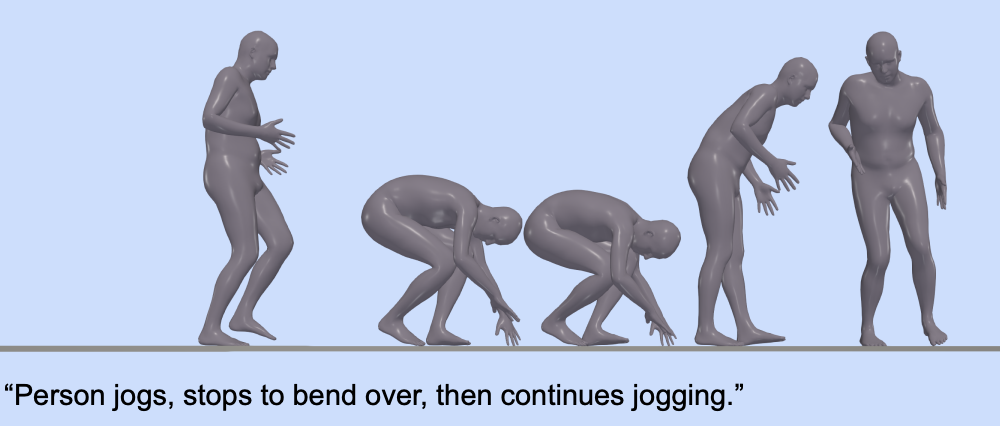
\includegraphics[width = 4in]{chapters/background_work/images/deep_learning_synthesis.png} 
  \caption{Deep Learning based synthesis} 
  \label{fig:deep_learning_synthesis} 
\end{figure}

\paragraph{Hybrid Workflows}
\label{ch:background_work:sign_language_synthesis:3d_techniques:avatar_animation:hybrid_workflows}

Hybrid worflows combine elements of manual keyframing, mocap retargeting, and procedural techniques to leverage the strengths of each method. By integrating these approaches, animators can achieve a balance between control, efficiency, and realism. For instance, an animator might use mocap data as a base and then refine specific movements with manual keyframes to enhance expressiveness. Additionally, procedural techniques can be applied to automate repetitive tasks or to ensure that certain \gls{posture_constraint}s are met dynamically during the animation process. Hybrid workflows offer a flexible and powerful workflow, allowing for the creation of complex animations that are both realistic and tailored to the specific needs of a project. Figure~\ref{fig:cascadeur} shows an example of a hybrid animation tool, Cascadeur.

\begin{figure} 
  \centering 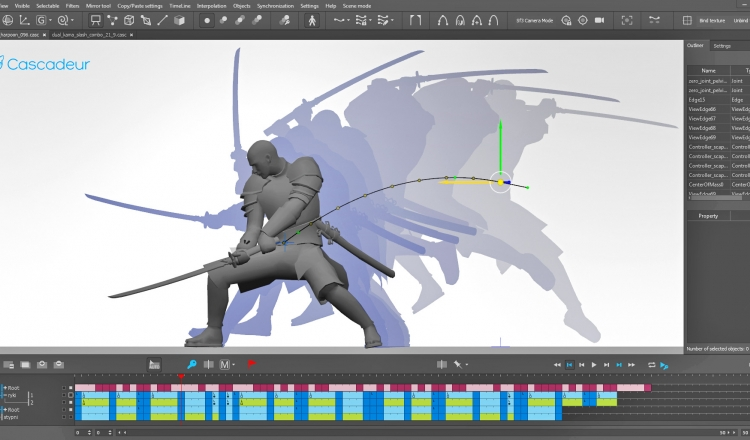
\includegraphics[width = 4in]{chapters/background_work/images/cascadeur.png} 
  \caption{Cascadeur hybrid animation tool} 
  \label{fig:cascadeur} 
\end{figure}

\paragraph{Face Animation}
\label{ch:background_work:sign_language_synthesis:3d_techniques:mesh_and_texture:face_animation}

This section explores rigging as well as animation of an avatar's face.

\paragraph{Face Rigging}
\label{ch:facial_expressions:related_work:face_rigging}

Face rigging is the process of creating a digital framework that allows for the animation of facial expressions. There are several approaches to face rigging, each with its own advantages and disadvantages.

\subparagraph{Blendshape-Based Rigging}
\label{ch:facial_expressions:related_work:face_rigging:blendshape_based_rigging}

Blendshape-based rigging involves creating a set of predefined facial shapes (blendshapes) that represent various expressions (figure~\ref{fig:blendshapes_smile}). Multiple versions of a mesh are stored to achieve this and interpolating between these meshes allows animators to blend between various expressions smoothly, such as smiling, frowning, or blinking. These blendshapes can be blended together in different proportions to create a wide range of facial expressions. However, it requires a large number of blendshapes to capture all possible expressions.

\begin{figure}[h]
  \centering
  \begin{subfigure}{0.3\linewidth} 
      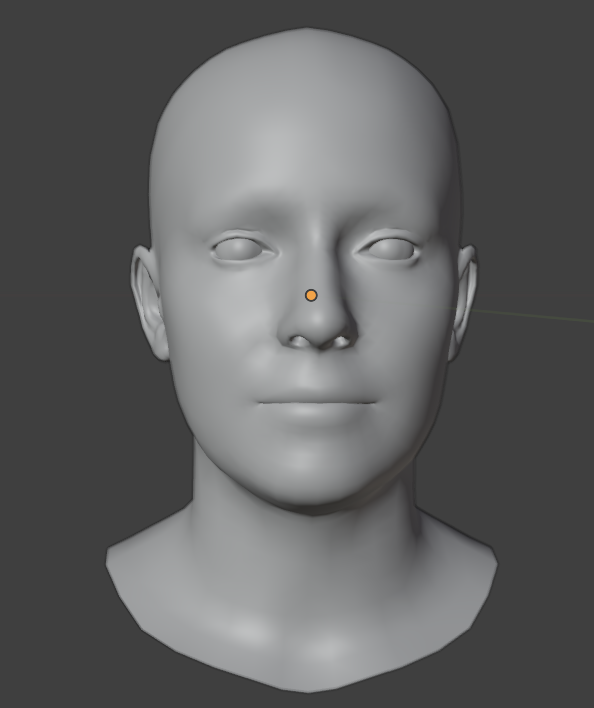
\includegraphics[width=\linewidth]{chapters/background_work/images/blendshapes_example/blendshapes_example_1.png} 
      \caption{Smile at 0} 
  \end{subfigure} 
  \hfill 
  \begin{subfigure}{0.3\linewidth} 
      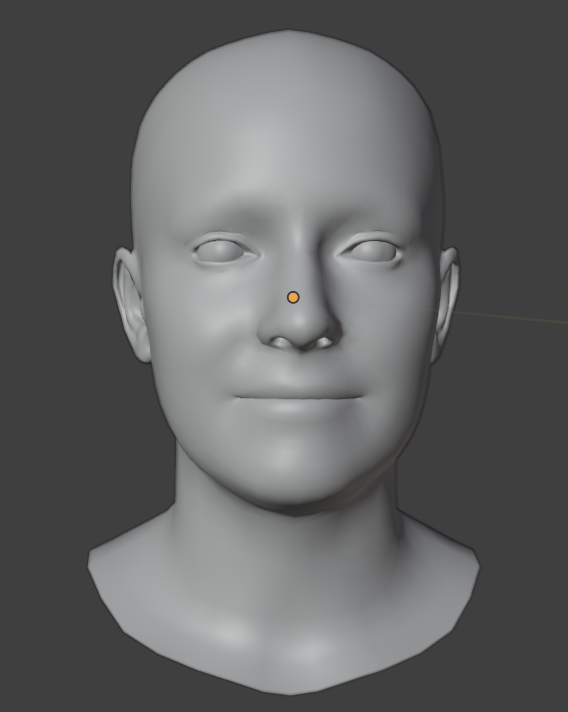
\includegraphics[width=\linewidth]{chapters/background_work/images/blendshapes_example/blendshapes_example_2.png} 
      \caption{Smile at 0.5} 
  \end{subfigure} 
  \hfill 
  \begin{subfigure}{0.3\linewidth} 
      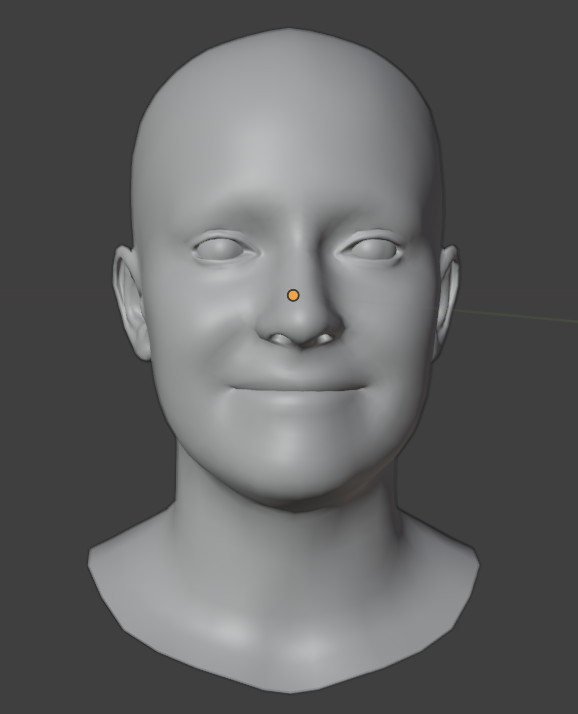
\includegraphics[width=\linewidth]{chapters/background_work/images/blendshapes_example/blendshapes_example_3.png} 
      \caption{Smile at 1} 
  \end{subfigure}
  \caption{Progression of smile using blendshapes from 0 to 1.0}
  \label{fig:blendshapes_smile}
\end{figure}

\subparagraph{Skeleton-Based Rigging}
\label{ch:facial_expressions:related_work:face_rigging:skeleton_based_rigging}

Skeleton-based rigging uses a hierarchical system of bones and joints to control facial movements (figure~\ref{ch:facial_expressions:fig:skeleton_based_rigging}). Each bone can control different parts of the face, such as the jaw, eyebrows, and eyelids. This offers more granular control but can be less intuitive than blendshapes for subtle expressions.

\begin{figure}
    \centering
    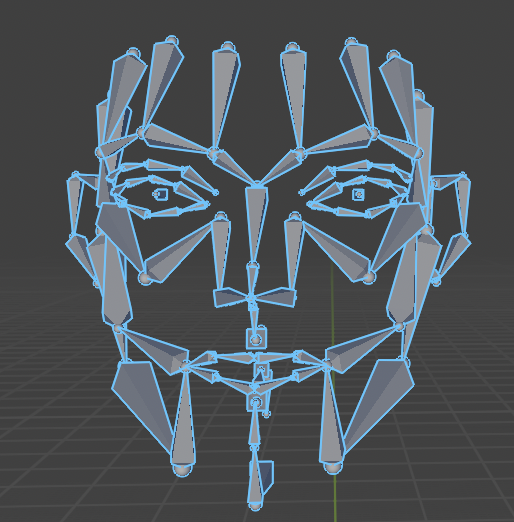
\includegraphics[width=0.8\textwidth]{chapters/background_work/images/facial_bones.png}
    \caption{Skeleton-based rigging for facial expressions}
    \label{ch:facial_expressions:fig:skeleton_based_rigging}
\end{figure}

\subparagraph{Hybrid Rigging}
\label{ch:facial_expressions:related_work:face_rigging:hybrid_rigging}

The use of blendshape-based rigging or skeleton-based rigging depends on the goal. More generally: 

\begin{itemize}
  \item \textbf{blendshapes}: Ideal for detailed and smooth transitions between expressions, but limited in flexibility.
  \item \textbf{Bones}: Provide granular control, better for interactive or dynamic facial animations but are more complex to set up and manage.
\end{itemize}

Usually, the two techniques are combined to offer greater flexibility and control.

\paragraph{Capturing Facial Expressions}
\label{ch:facial_expressions:related_work:face_rigging:capture}

Facial expressions can be captured manually or through performance-based techniques.

\subparagraph{Manual Keyframing}
\label{ch:facial_expressions:related_work:face_rigging:capture:manual_keyframing}

Manual keyframing is a foundational animation technique, where animators manually set key poses (figure~\ref{ch:facial_expressions:fig:keyframing}). It is effective but may struggle to capture the variability required in \gls{sl} synthesis.

\begin{figure}
    \centering
    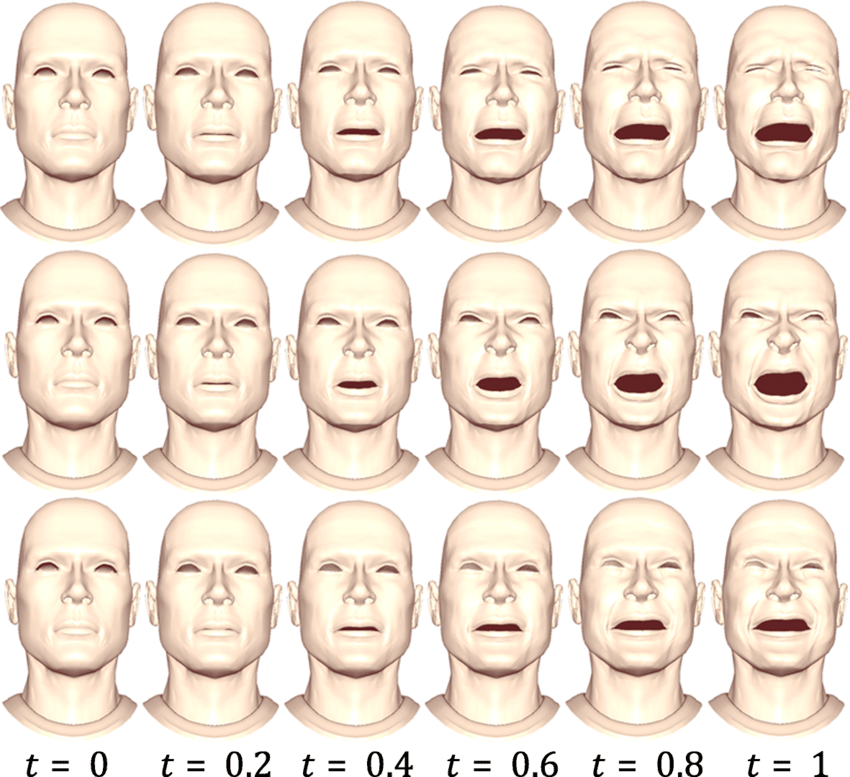
\includegraphics[width=0.8\textwidth]{chapters/background_work/images/facial_keyframing.png}
    \caption{Keyframing process, showing how key poses are set and interpolated to create a continuous animation.}
    \label{ch:facial_expressions:fig:keyframing}
\end{figure}

\subparagraph{Performance-Based Motion Capture}
\label{ch:facial_expressions:related_work:face_rigging:capture:performance_based_motion_capture}

Performance-based motion capture captures human facial movements and uses this data to animate digital avatars. Tools like Apple's ARKit (figure~\ref{ch:facial_expressions:fig:motion_capture}) are examples of this approach.

\begin{figure}
    \centering
    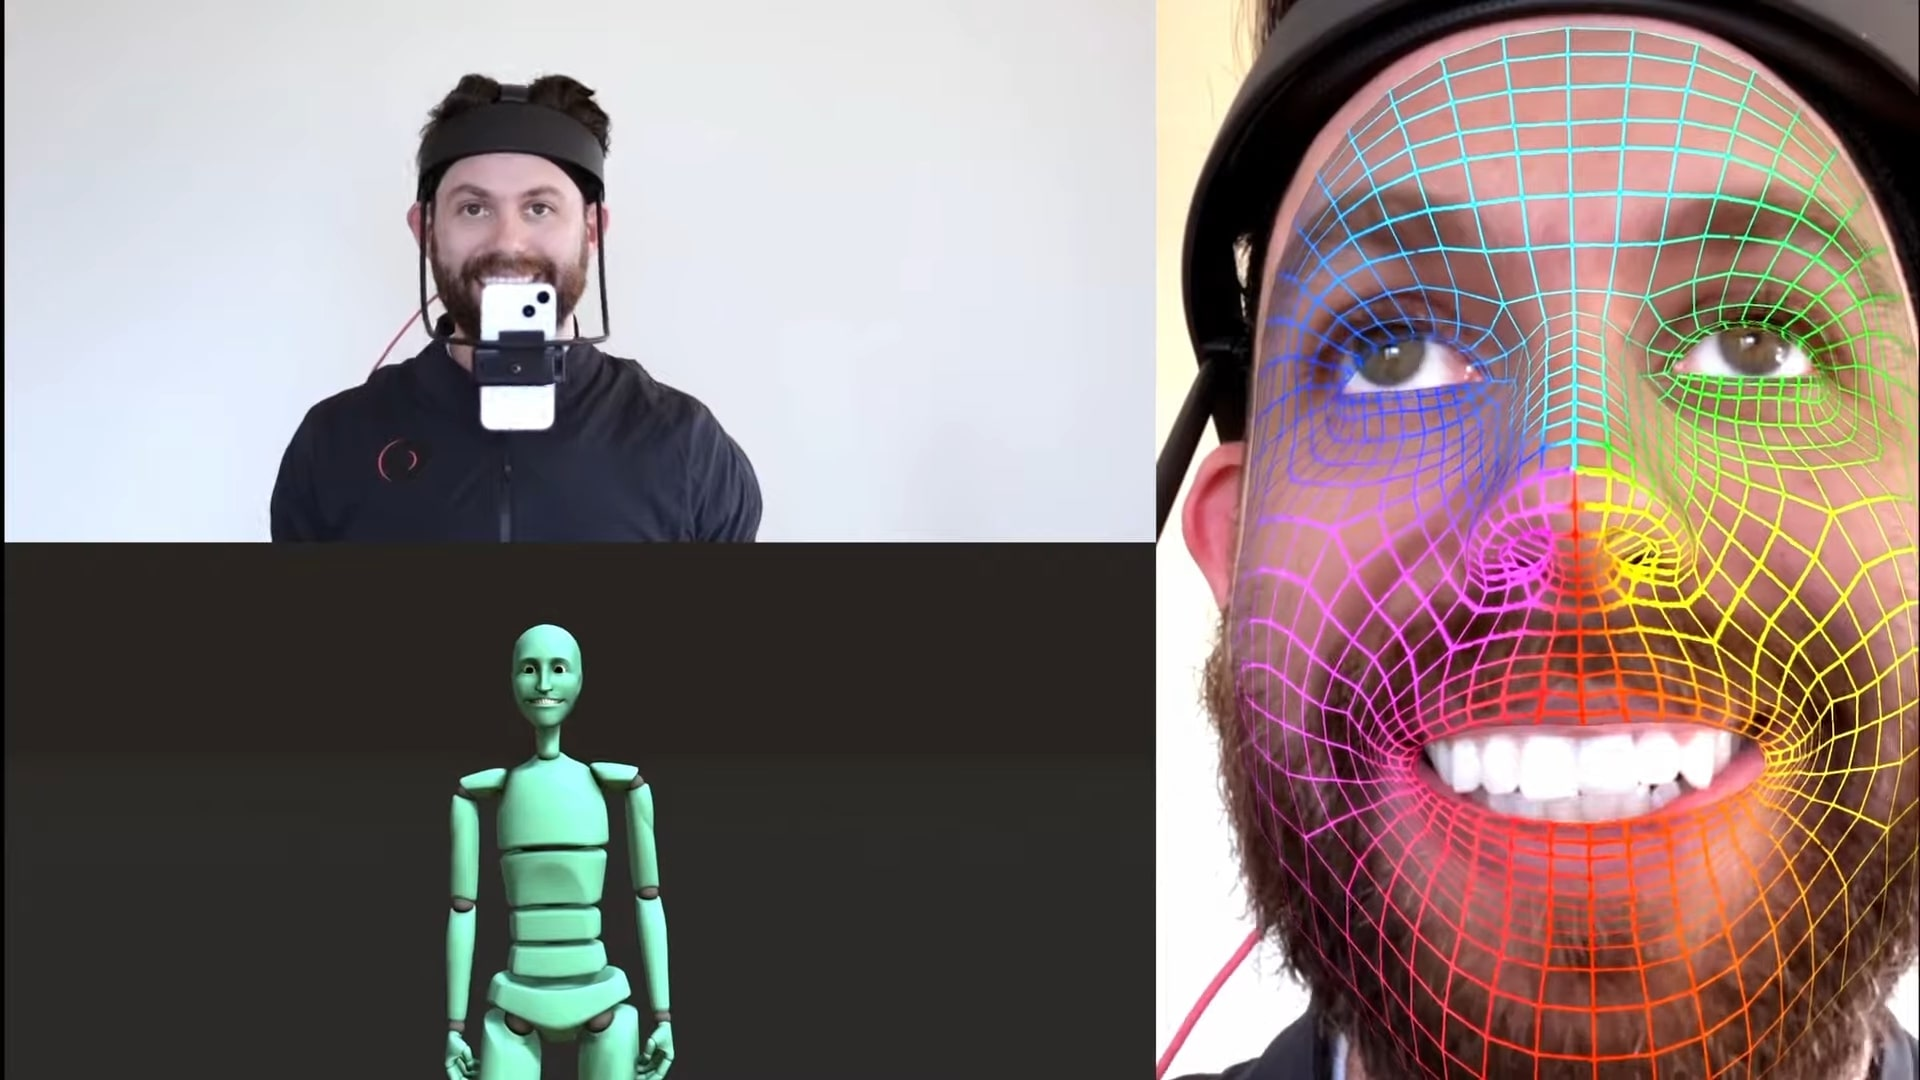
\includegraphics[width=0.8\textwidth]{chapters/background_work/images/facial_motion_capture.jpg}
    \caption{Performance-based facial animation using Apple's ARKit}
    \label{ch:facial_expressions:fig:motion_capture}
\end{figure}

\subparagraph{Facial Expressions Synthesis}
\label{ch:background_work:sign_language_synthesis:3d_techniques:face_animation:facial_expressions_synthesis}

Most facial expression research is motivated by synthesis from voice signals. These methods are generally categorized into lip-sync techniques~\cite{yousaidthat, talkingface, lipmovements, lipsyncexpert}, which align mouth movements with audio, and full-face expression synthesis~\cite{eskimez, greenwood18, controllable_facial_synth}. Some approaches model speaking style with 3D animation parameters~\cite{cudeiro}, or create generalized latent audio expressions combined with a person-specific 3D model~\cite{FLAME}. Related work, MakeItTalk~\cite{Yang:2020:MakeItTalk}, introduces a two-stage deep learning model that predicts facial landmark displacements based on audio input, followed by an image-to-image translation method to generate the final facial expression. 

\subparagraph{Emotion Recognition}
\label{ch:facial_expressions:related_work:emotion_recognition}

Emotion recognition systems use machine learning algorithms to analyze facial features and identify the underlying emotional state. The most common approach to define emotions is Ekman's Facial Action Coding System (FACS)~\cite{ekman1978facial}, which categorizes facial expressions into action units (AUs) (figure~\ref{ch:facial_expressions:fig:action_units}). EMOCA~\cite{danvevcek2022emoca} uses 3D face reconstruction to capture emotional expressions accurately, significantly improving expression quality over previous methods.

\begin{figure}
    \centering
    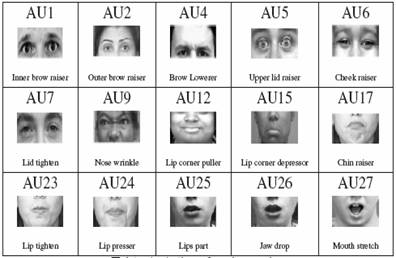
\includegraphics[width=0.8\textwidth]{chapters/background_work/images/action_units.jpg}
    \caption{Facial Action Coding System (FACS) action units}
    \label{ch:facial_expressions:fig:action_units}
\end{figure}

\paragraph{Uncanny Valley}
\label{ch:background_work:sign_language_synthesis:3d_techniques:avatar_animation:uncanny_valley}

The Uncanny Valley is a concept in robotics and 3D animation that describes the discomfort or eeriness people feel when they encounter a humanoid figure that is very close to, but not quite, human-like. This phenomenon was first identified by roboticist Masahiro Mori in 1970.

As avatars become more realistic in appearance and movement, they initially become more appealing and relatable. However, there is a point at which the avatar becomes almost, but not perfectly, human-like, causing a sense of unease or revulsion in the observer. This dip in the graph of familiarity versus human likeness is known as the Uncanny Valley.

Figure~\ref{fig:uncanny_valley_graph} illustrates the Uncanny Valley effect, showing how an increase in human likeness can lead to a dip in emotional response before rising again as realism improves.

\begin{figure}
  \centering
  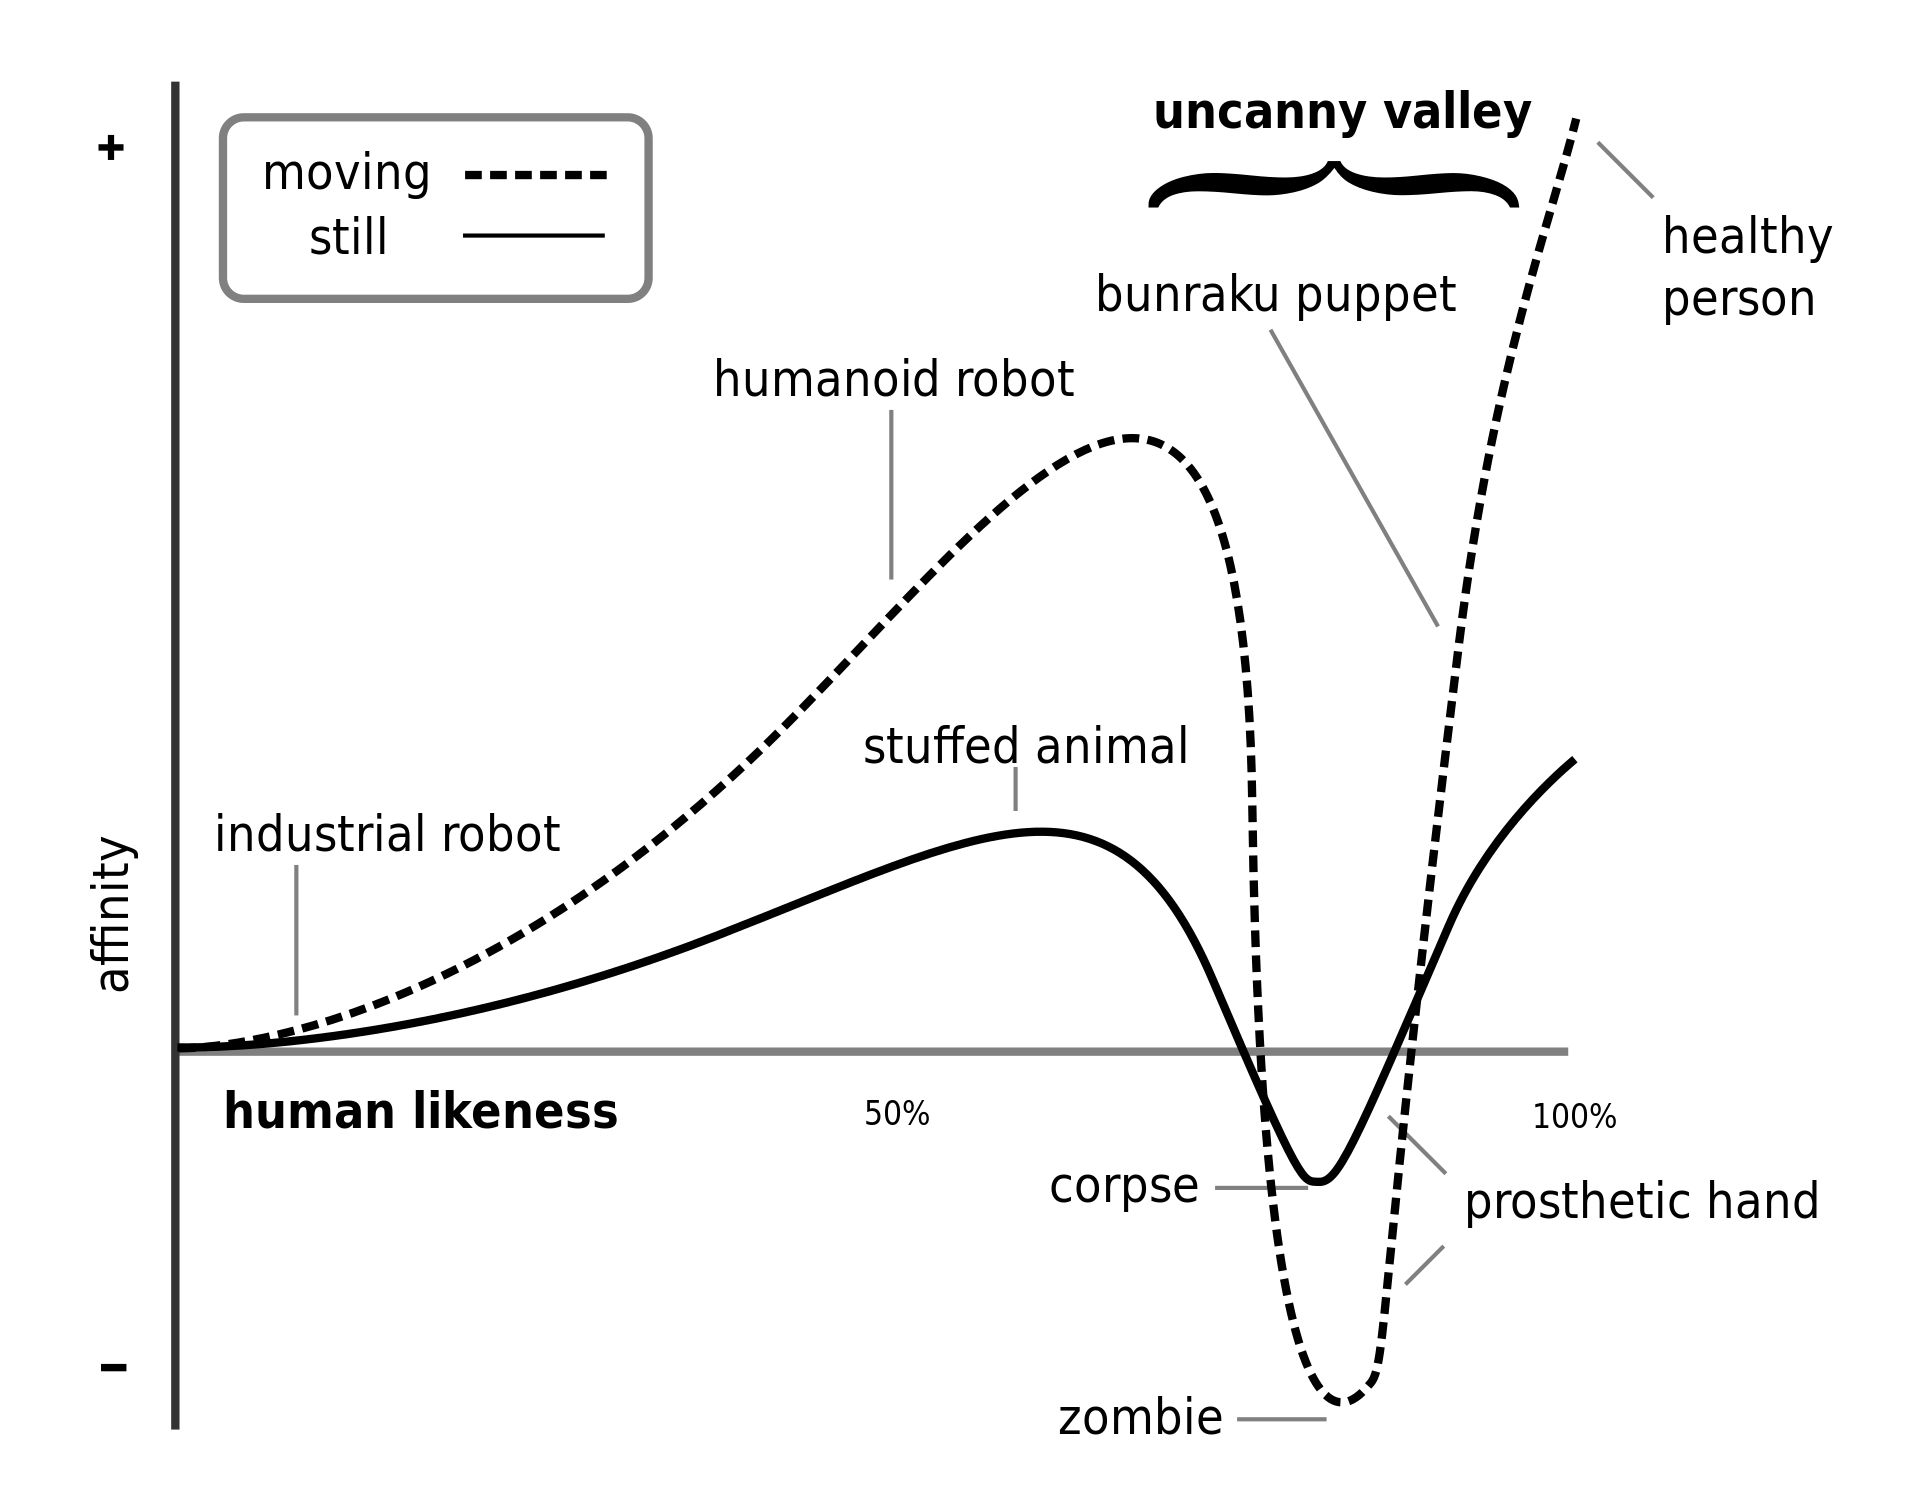
\includegraphics[width = 2.5in]{chapters/background_work/images/uncanny_valley_graph.png}
  \caption{Graph illustrating the Uncanny Valley effect}
  \label{fig:uncanny_valley_graph}
\end{figure}

The factors contributing to the Uncanny Valley effect often include:

\begin{itemize}
  \item \textbf{Facial Expressions}: Subtle imperfections in facial expressions, such as unnatural eye movements or lifeless smiles, can make the avatar appear creepy or unsettling.
  \item \textbf{Movement}: Non-human-like movements, jerky motions, or slight deviations from natural human motion can heighten the uncanny effect.
  \item \textbf{Texture and Skin Tone}: Inconsistent skin textures, overly smooth surfaces, or unrealistic lighting and shading can make an avatar appear artificial.
  \item \textbf{Eye Contact}: The eyes are critical in conveying emotions and life. Any deviation in eye movement, blink patterns, or focus can make an avatar look eerie.
\end{itemize}

Understanding and mitigating the Uncanny Valley effect is crucial for animators and developers aiming to create realistic and relatable avatars. One way to avoid the Uncanny Valley could be to use stylized avatars, which are intentionally designed to deviate from realism and have a unique aesthetic. Another approach is to keyframe more information in the animations themselves, ensuring that movements and expressions are as natural and lifelike as possible.

\subsubsection{SL Synthesis Systems}
\label{ch:background_work:sign_language_synthesis:3d_techniques:sign_language_synthesis_systems}

In the context of \gls{sl} synthesis, several advanced systems have been developed to automate the generation and animation of \gls{sl}.

\paragraph{JASigning}
\label{ch:background_work:sign_language_synthesis:3d_techniques:sign_language_synthesis_systems:jasigning}

JASigning is an advanced \gls{sl} avatar system developed within the scope of the ViSiCAST and eSIGN projects. It enables the automatic generation and animation of \gls{sl} through a predefined set of gestures and animations. These gestures can be dynamically combined to form coherent \gls{sl} sentences. JASigning is designed to support multiple \gls{sl}s and integrates with text-to-sign translation systems. The system uses HamNoSys in the form of an XML representation to describe signs and their components. JASigning has been used in various applications, including educational tools, communication aids, and virtual avatars.

Figure~\ref{fig:jasigning} shows an example of the JASigning system in action.

\begin{figure} 
  \centering \includegraphics[width = 2.5in]{chapters/background_work/images/jasigning.png} 
  \caption{JASigning} 
  \label{fig:jasigning} 
\end{figure}

\paragraph{EMBR}
\label{ch:background_work:sign_language_synthesis:3d_techniques:sign_language_synthesis_systems:embr}

Unlike the previous models, EMBR (Embodied Agents Behaviour Realizer) Script is a scripting language used to control virtual characters in general and is not restricted to \gls{sl} avatars. However, EMBRScript allows for animation specification through a sequence of key poses, each defined at specific time points for a precise specification of body movements, facial expressions, and other actions. This also makes it usable to describe signs with synthesis using an avatar in mind.

EMBR is a real-time animation engine engineered to produce expressive gestures and \gls{sl} for virtual avatars. EMBR facilitates precise control over avatar movements, encompassing hand shapes, facial expressions, and body postures critical for accurate \gls{sl} depiction. The framework supports scripting and integrates with various input modalities, such as text or motion capture data, to generate realistic and contextually appropriate \gls{sl} animations. EMBR's flexibility and adaptability make it a valuable tool in research settings, particularly for studies focused on the nuances of non-verbal communication and the development of nuanced, context-sensitive gestures.

\paragraph{Synthesis based on Generative Models}
\label{ch:background_work:sign_language_synthesis:3d_techniques:sign_language_synthesis_systems:synthesis_based_on_generative_models}

Generative models have shown promise in \gls{sl} synthesis by learning the underlying structure of \gls{sl} data and generating new animations. These models can be trained on large datasets of \gls{sl} videos to capture the complex relationships between linguistic input and \gls{sl} output. Some popular generative models used in \gls{sl} synthesis include:

\subparagraph{Gloss based}
\label{ch:background_work:sign_language_synthesis:3d_techniques:sign_language_synthesis_systems:synthesis_based_on_generative_models:gloss_based}

\gls{sl} animation from text focuses on generating realistic \gls{sl} videos from written text. The process involves text-to-gloss conversion, gloss-to-pose generation, and pose-to-sign rendering. Recent approaches utilize neural networks and generative models to enhance animation fluidity and realism. One method uses dictionary examples and a codebook of signs to create continuous \gls{sl} sequences, incorporating both manual and non-manual features. However, challenges remain in annotating the data and training the models effectively, particularly in the production of natural hand and facial movements.

\subparagraph{SignAvatars}
\label{ch:background_work:sign_language_synthesis:3d_techniques:sign_language_synthesis_systems:synthesis_based_on_generative_models:signavatars}

The SignAvatars~\cite{yu2023signavatars} dataset introduces a large-scale, multi-prompt 3D \gls{sl} motion dataset with 70,000 videos and 8.34 million frames from 153 signers. It includes isolated and continuous signs, annotated with 3D meshes and biomechanically-valid poses. The dataset supports tasks such as 3D \gls{sl} recognition and production from text scripts, individual words, and HamNoSys notation. A novel annotation pipeline ensures accurate 3D holistic annotations. Evaluation metrics indicate significant improvements in generating natural and consistent 3D \gls{sl} animations from diverse textual inputs using models like Sign-VQVAE.

\subparagraph{Sgnify}
\label{ch:background_work:sign_language_synthesis:3d_techniques:sign_language_synthesis_systems:synthesis_based_on_generative_models:sgnify}

Recent advancements in 3D reconstruction from \gls{sl} videos~\cite{Forte_2023_CVPR}, focusing on isolated signs. SGNify leverages linguistic priors, such as hand-pose symmetry and invariance, to enhance the accuracy of hand-pose estimation in challenging \gls{sl} videos. The approach outperforms existing 3D body-pose estimation methods, particularly in handling self-occlusions and motion blur. Quantitative and perceptual evaluations demonstrate that SGNify's reconstructions are more natural and comprehensible than previous methods, achieving sign recognition rates comparable to original video performances.

\subsubsection{AZee based}
\label{ch:background_work:sign_language_synthesis:3d_techniques:sign_language_synthesis_systems:azee_based}

This subsection explores AZee-based \gls{sl} synthesis systems, highlighting advancements in avatar animation using both pre-animated and low-level synthesis techniques.

\paragraph{Paula}
\label{ch:background_work:sign_language_synthesis:3d_techniques:sign_language_synthesis_systems:azee_based:paula}

The Paula avatar system, integrated with AZee linguistic descriptions, represents a significant advancement in \gls{sl} synthesis. AZee provides a robust, high-level framework that encodes both form and functional aspects of \gls{sl}, while Paula ensures the translation of these descriptions into fluid, human-like motion. This combination addresses earlier challenges in \gls{sl} avatars, particularly the difficulty in creating natural and expressive signing.

Initial work focused on developing a pipeline that connects AZee's abstract linguistic input directly to avatar animation~\cite{filhol2017synthesizing}. This method enabled the synthesis of natural signing by leveraging the structure of \gls{sl} discourse, focusing on the transitions between signs, which had previously been overlooked~\cite{mcdonald2021natural}. Smooth and context-aware transitions were found to be essential for creating fluid and cohesive animations, as these movements contribute significantly to the natural pacing of \gls{sl} discourse.

An important challenge addressed by the system is the synthesis of productive signing forms such as classifier predicates and size and shape specifiers. These highly variable constructs had previously been difficult to animate, as they cannot be pre-recorded or standardized like frozen signs~\cite{filhol2020synthesis}. By defining a set of flexible rules that cover a wide range of proform constructs, the system allows for the natural generation of these elements. This flexibility enables the avatar to handle both the positioning and movement of objects in space with greater accuracy and variability, which is crucial for conveying meaning in \gls{sl}.

As the system matured, further refinements focused on capturing the subtleties of movement that enhance the realism of \gls{sl} animation. For example, placing objects or classifiers in space involves more than simply positioning the hand; it requires dynamic variations based on context~\cite{mcdonald2019fine}. The avatar adapts its motion depending on whether it is placing a single object, multiple objects consecutively, or a set of items. In each case, the timing, pacing, and pauses between movements vary, contributing to more authentic animations.

Another major area of improvement has been the handling of facial expressions and non-manual signals. Facial movements are critical for conveying both grammatical and affective information in \gls{sl}. However, they are particularly challenging to reproduce on avatars due to the complexity of human facial anatomy. Recent developments have improved the range of facial expressions the Paula avatar can produce, incorporating fine details such as wrinkles to enhance clarity and legibility, particularly when viewed on smaller screens~\cite{johnson2021towards}. This attention to detail ensures that the avatar can effectively communicate nuanced facial expressions, which are essential for the overall comprehension of signing.

The Paula system also employs a hierarchical model that organizes signing into larger linguistic structures, allowing for smoother, more coherent animations~\cite{filhol2018extending}. This approach helps the avatar synthesize more natural-looking movement by considering the overall discourse, rather than focusing solely on individual signs or gestures. For example, geometric templates are used to position proforms—abstract representations of objects—in the signing space. These templates provide a consistent framework for handling spatial relations, ensuring that the avatar can dynamically adjust its movements across various signing scenarios.

\begin{figure}
    \centering \includegraphics[width = 2.5in]{chapters/background_work/images/azee_template_example.png}
    \caption{AZee Templates used by the Paula avatar for positioning proforms in signing space}
    \label{fig:azee_geo_template_example}
\end{figure}

By focusing on higher-level linguistic structures, the system avoids relying on a fixed set of predefined points, which is critical for capturing the inherent variability and dynamism of \gls{sl}. This method allows the Paula avatar to produce more expressive and flexible animations, particularly in scenarios involving spatial descriptions or interactions with multiple objects.

Overall, the combination of AZee’s linguistic richness with Paula’s realistic motion synthesis offers a robust solution for \gls{sl} animation. By addressing both the high-level discourse structure and the finer details of movement, the system produces animations that are not only accurate but also natural and engaging. However, even though Paula integrates AZee descriptions with pre-recorded motion data, it cannot synthesize from low-level AZee descriptions directly. This poses complexity in the system's scalability and flexibility, as the animations have to be animated by artists. This is where the low-level synthesizer for AZee comes in.

\paragraph{Low-level synthesizer for AZee}
\label{ch:background_work:sign_language_synthesis:3d_techniques:sign_language_synthesis_systems:azee_based:low_level_synthesizer_for_azee}

A low-level synthesizer for AZee~\cite{nunnari2018animating} has already been developed to address the limitations of the top-down approach used by Paula. The low-level synthesizer generates animations directly from AZee's \gls{azee_score}, allowing for a better scalability in \gls{sl} synthesis since the linghuists input can be directly used to generate animations instead of relying on artists.

\subparagraph{Animated Score}
\label{ch:background_work:sign_language_synthesis:3d_techniques:sign_language_synthesis_systems:azee_based:low_level_synthesizer_for_azee:animated_score}

The Animated Score is a \emph{flattened} representation of the AZee \gls{cstr_score}. To understand this better, let's consider (figure~\ref{fig:azee_score_armoire_combined}) the \gls{azee_score} for the description of the sign \emph{:armoire} (\emph{cupboard} in \gls{lsf}).

\begin{figure}[h]
  \centering
  \includegraphics[width=0.9\textwidth]{chapters/background_work/images/azee_score_armoire_combined.png}
  \caption{AZee Synced Score generated from the low-level AZee description.}
  \label{fig:azee_score_armoire_combined}
\end{figure}

Although AZee is multi-track by nature (where the lingusit has the ability to crate the track), the low-level AZee synthesizor uses an \emph{Animated Score} which is a flattened version of an AZee Synced Score, where all the tracks are merged into a single track. This flattening is done by collecting all the \gls{posture_constraint}s for each frame and applying them to the corresponding bone rotations during animation. Figure~\ref{fig:azee_score_armoire_combined} visualizes this flattening process shows the flattened version of the AZee Synced Score.

During evaluation, the low-level synthesizer creates postures for each of the frame using this Animated Score. For this, they used the algorithm~\ref{alg:trimmed_constraint_based_optimization} for the pose optimization for each of the constraints to generate the postures. 

\begin{algorithm}
  \caption{Constraint-Based Optimization for Posture Synthesis}
  \label{alg:trimmed_constraint_based_optimization}
  \begin{algorithmic}[1]
  \Require $\text{PostureConstraints} \ \mathit{posture\_constraint}$, $\text{Object} \ \mathit{armature\_object}$
  \Ensure Armature object is posed according to the constraints
  
  \State \textbf{Initialize:} $i \gets 0$
  \State $distance\_threshold \gets \mathit{bpy.context.scene.azee\_ik\_site\_distance\_threshold}$
  \State $angle\_threshold \gets \mathit{bpy.context.scene.azee\_ik\_bone\_rot\_angle\_threshold \times \pi / 180}$
  \State $max\_iterations \gets \mathit{bpy.context.scene.azee\_ik\_max\_iterations}$
  
  \While{$i < max\_iterations$}
      \State \textbf{Apply Constraints:} \textsc{ApplyPositionConstraint}($\mathit{posture\_constraint}$), \textsc{ApplyOrientConstraints}($\mathit{posture\_constraint}$)
      \State \textbf{Compute Offsets:} $place\_distance, orient\_angles \gets \textsc{ComputeDistance}(\mathit{posture\_constraint})$
      \If {$\mathit{place\_distance} < \mathit{distance\_threshold}$ \textbf{and} $\max(\mathit{orient\_angles}) < \mathit{angle\_threshold}$}
          \State \textbf{Break:} \textbf{end while}
      \EndIf
      \State $i \gets i + 1$
  \EndWhile
  
  \Procedure{ApplyPositionConstraint}{$\mathit{posture\_constraint}$}
      \If {$\mathit{posture\_constraint.place\_constraint} \neq \text{None}$}
          \State \textbf{Apply IK:} \textsc{ApplyIKConstraint}($\mathit{posture\_constraint.place\_constraint.site\_pose\_bone}$, 
          \textsc{CreateTemporaryTarget}($\mathit{posture\_constraint.place\_constraint.target\_vect}$), \textit{position})
      \EndIf
  \EndProcedure
  
  \Procedure{ApplyOrientConstraints}{$\mathit{posture\_constraint}$}
      \ForAll {$orient\_constraint \in \mathit{posture\_constraint.orient\_constraints}$}
          \State \textbf{Apply IK:} \textsc{ApplyIKConstraint}($orient\_constraint.pose\_bone$, 
          \textsc{CreateTemporaryTarget}($orient\_constraint.get\_target\_quaternion()$), \textit{rotation}, 
          $orient\_constraint.get\_axis\_relaxation\_mask()$)
      \EndFor
  \EndProcedure
  
  \Procedure{ComputeDistance}{$\mathit{posture\_constraint}$}
      \State \Return \textsc{ComputeDistanceFromOffset}(\textsc{ComputePlaceOffset}($\mathit{posture\_constraint}$)), 
      \textsc{ComputeAnglesFromOffsets}(\textsc{ComputeOrientOffsets}($\mathit{posture\_constraint}$))
  \EndProcedure
  \end{algorithmic}
\end{algorithm}

For the pose optimization, the algorithm~\ref{alg:trimmed_constraint_based_optimization} uses a distance threshold and an angle threshold to determine when the optimization has converged. The algorithm iterates through the constraints, applying them to the armature object and computing the offsets. If the distance and angle thresholds are met, the optimization process is terminated and the posture is keyframed. This process is repeated for each frame in the Animated Score, generating a sequence of keyframes that represent the desired animation. The synthesizer is implemented as an add-on in Blender and uses the iTaSC solver to solve the \gls{ik} problems. Figure \ref{fig:armoire_low_level} shows the synthesized animation for the sign \emph{:armoire} using the low-level synthesizer.

\begin{figure}
  \centering
  \includegraphics[width=0.8\textwidth]{chapters/background_work/images/armoire_low_level.png}
  \caption{Synthesized animation for the sign \emph{:armoire} using the low-level synthesizer.}
  \label{fig:armoire_low_level}
\end{figure}

Even though this approach allows a better coverage using AZee descriptions since it can directly generate animations from the linguists input without relying on artists. It is in-extensible to be used with pre-animated motion data blocks for larger sequences since the flattened representation does not contain the original reference of the corresponding animation block on the timeline. More importantly, it generates robotic animations since it does not consider the nuances of natural human motion. This work therefore is the other side of the coin to a high-level synthesis technique like Paula, which are hindered by the labor-intensive nature of hand-crafted animations.

\paragraph{Granularity of \gls{sl} Synthesis}
\label{ch:background_work:sign_language_synthesis:3d_techniques:sign_language_synthesis_systems:granularity_of_sl_synthesis}

The granularity of \gls{sl} synthesis refers to the level of detail at which signs are represented and animated. High-level synthesis techniques focus on capturing the overall structure and meaning of signs, often using abstract linguistic descriptions to guide the animation process. These methods are efficient for generating coherent and contextually appropriate animations but may lack the fine-grained control needed to produce nuanced and expressive signing.

In contrast, low-level synthesis techniques aim to capture the detailed movements and articulations of signs, focusing on the precise positioning and orientation of body parts. These methods offer greater flexibility and realism in animation but require more manual intervention and expertise to produce accurate and natural-looking signing.

This distinction between high-level and low-level synthesis reflects a trade-off between efficiency and expressiveness in \gls{sl} animation and forms the basis of this thesis.

\section{Conclusion}
\label{ch:background_work:conclusion}

To summarize:

\begin{itemize} 
  \item Linear systems for \gls{sl} representation are limited in their expressive capacity and fail to capture the complexity of natural \gls{sl}.
  \item Non-linear systems provide better coverage and more accurately reflect the nuances of \gls{sl}.
  \item Systems like Paula and AZee, which incorporate both form and functional aspects, offer a promising approach but are hindered by the labor-intensive nature of hand-crafted animations.
  \item There is a need for low-level synthesis techniques to complement these high-level models, allowing for greater flexibility and coverage.
  \item Existing low-level synthesis approaches, such as those using \gls{ik} solvers, provide a foundation but require further development to fully support the diverse requirements of \gls{sl} animation.
  \item By addressing these gaps, we aim to advance the state of \gls{sl} synthesis, making it more scalable and capable of generating natural and expressive animations.
\end{itemize}

Throughout this chapter, we have introduced, defined, and discussed a variety of concepts from three research areas that are key to this thesis: \textit{\gls{sl} representation}, \textit{avatars}, and \textit{\gls{sl} synthesis}. In the rest of the manuscript, we heavily rely on many of these concepts to investigate ways in which models for \gls{sl} synthesis can progressively learn and improve using newer techniques.

In Chapter~\ref{ch:avatar_creation_pose_synthesis} and chapter~\ref{ch:multi_track}, we study ways to create and rig a \gls{sl} avatar as well as explore multi-track timeline generation from AZee respectively. Chapter~\ref{ch:intermediate_blocks_pose_correction} dives deeper into reusing animations using template matching as well as generating better poses for synthesis. Additionally, the studies presented in chapter~\ref{ch:facial_expressions} discuss means to synthesize facial expressions for \gls{sl}. Lastly, Chapter~\ref{ch:conclusion} concludes the manuscript by summarizing the findings and discussing future research directions.

\end{document}
